%%%%%%%%%%%%%%%%%%%%%%%%%%%%%%%%%%%%%%%%%
% Beamer Presentation
% LaTeX Template
% Version 1.0 (10/11/12)
%
% This template has been downloaded from:
% http://www.LaTeXTemplates.com
%
% License:
% CC BY-NC-SA 3.0 (http://creativecommons.org/licenses/by-nc-sa/3.0/)
%
%%%%%%%%%%%%%%%%%%%%%%%%%%%%%%%%%%%%%%%%%

%----------------------------------------------------------------------------------------
%	PACKAGES AND THEMES
%----------------------------------------------------------------------------------------
\documentclass{beamer}

\mode<presentation> {

% The Beamer class comes with a number of default slide themes
% which change the colors and layouts of slides. Below this is a list
% of all the themes, uncomment each in turn to see what they look like.

% \usetheme{default}
%\usetheme{AnnArbor}
%\usetheme{Antibes}
%\usetheme{Bergen}
%\usetheme{Berkeley}
%\usetheme{Berlin}
%\usetheme{Boadilla}
% \usetheme{CambridgeUS}
% \usetheme{Copenhagen}
\usetheme{Darmstadt}
%\usetheme{Dresden}
%\usetheme{Frankfurt}
%\usetheme{Goettingen}
%\usetheme{Hannover}
%\usetheme{Ilmenau}
%\usetheme{JuanLesPins}
%\usetheme{Luebeck}
% \usetheme{Madrid}
%\usetheme{Malmoe}
%\usetheme{Marburg}
%\usetheme{Montpellier}
%\usetheme{PaloAlto}
%\usetheme{Pittsburgh}
%\usetheme{Rochester}
%\usetheme{Singapore}
%\usetheme{Szeged}
%\usetheme{Warsaw}

% For adding page number in "Darmstadt" theme
\addtobeamertemplate{navigation symbols}{}{%
    \usebeamerfont{footline}%
    \usebeamercolor[fg]{footline}%
    \hspace{1em}%
    \insertframenumber/\inserttotalframenumber
}

% As well as themes, the Beamer class has a number of color themes
% for any slide theme. Uncomment each of these in turn to see how it
% changes the colors of your current slide theme.

%\usecolortheme{albatross}
%\usecolortheme{beaver}
%\usecolortheme{beetle}
%\usecolortheme{crane}
%\usecolortheme{dolphin}
%\usecolortheme{dove}
%\usecolortheme{fly}
%\usecolortheme{lily}
%\usecolortheme{orchid}
%\usecolortheme{rose}
%\usecolortheme{seagull}
%\usecolortheme{seahorse}
%\usecolortheme{whale}
%\usecolortheme{wolverine}

%\setbeamertemplate{footline} % To remove the footer line in all slides uncomment this line
%\setbeamertemplate{footline}[page number] % To replace the footer line in all slides with a simple slide count uncomment this line

%\setbeamertemplate{navigation symbols}{} % To remove the navigation symbols from the bottom of all slides uncomment this line
}

% tikz and flowchart
\usepackage{tikz}
\usetikzlibrary{shapes.geometric, arrows}

\usepackage{transparent}
\usepackage{natbib}
\usepackage{overpic}
\usepackage{subfig}
\usepackage{graphicx} % Allows including images
\usepackage{booktabs} % Allows the use of \toprule, \midrule and \bottomrule in tables
\definecolor{olivegreen}{RGB}{34,139,34}
\definecolor{darkorange}{RGB}{255,140,0}
%----------------------------------------------------------------------------------------
%	TITLE PAGE
%----------------------------------------------------------------------------------------

\title[CR proton from $\gamma$-ray Earth's Limb]{Indirect measurement of cosmic-ray proton spectrum using Earth's $\gamma$-ray data from {\it Fermi} Large Area Telescope }
% \logo{
\includegraphics[height=0.75cm]{santa}}
\author[P. Payoungkhamdee]{
  Patomporn Payoungkhamdee$^{\dagger}$ \\
  {
    \small Supervised by \\
    Asst. Prof. Warit Mitthumsiri$^{\dagger}$ and Prof. David Ruffolo$^{\dagger}$
  }
} % Your name
\institute[MU] % Your institution as it will appear on the bottom of every slide, may be shorthand to save space
{
  $^{\dagger}$Department of Physics, Faculty of Science, Mahidol University \\ % Your institution for the title page
\medskip
\textit{patomporn.pay@gmail.com} % Your email address

}
\date[14 June 2021]{Master thesis defend \\ 14 June 2021} % Date, can be changed to a custom date

\newcommand{\nologo}{\setbeamertemplate{logo}{}}

\begin{document}

{\nologo
\begin{frame}
\titlepage % Print the title page as the first slide
\end{frame}
}

\begin{frame}
\frametitle{Overview} % Table of contents slide, comment this block out to remove it
\tableofcontents % Throughout your presentation, if you choose to use \section{} and \subsection{} commands, these will automatically be printed on this slide as an overview of your presentation
\end{frame}

%----------------------------------------------------------------------------------------
%	PRESENTATION SLIDES
%----------------------------------------------------------------------------------------


%------------------------------------------------
%      Objectives
%------------------------------------------------
\section{Objectives}
% \section{Objectives} % Sections can be created in order to organize your presentation into discrete blocks, all sections and subsections are automatically printed in the table of contents as an overview of the talk

%---- our point ---
\begin{frame}
\frametitle{Objective}
\begin{itemize}
  \item To measure CR proton spectrum between 60 GV - 2 TV using
  Earth's $\gamma$-ray data from \textit{Fermi}-LAT
  through the interaction model by \cite{K&Omodel}
  \item To test if the \textit{Fermi}-LAT data confirm the
  spectral break at around 340 GV as observed by some experiments
\end{itemize}
\end{frame}


%------------------------------------------------
%    1 ) Introduction
%------------------------------------------------
% \section{Introduction}
% \section{Background}
%---- 
% \begin{frame}
% \frametitle{Introduction}
% \end{frame}

%---- 
% \begin{frame}
%   \begin{figure}
%   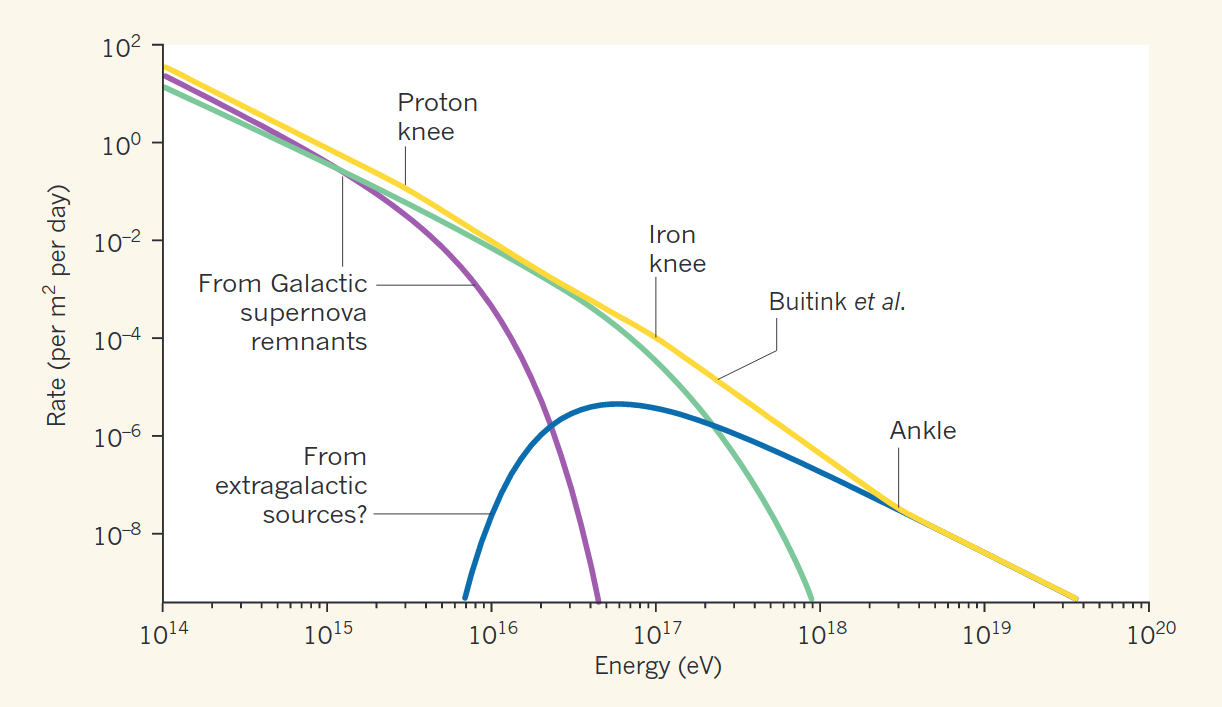
\includegraphics[width=\textwidth]{figure/andrew_superposition.png}
%     % 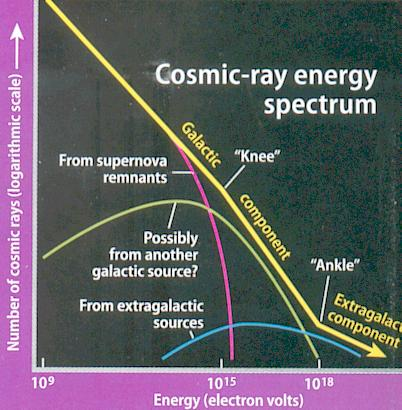
\includegraphics[height=0.7\textheight, width=0.9\textwidth]{CRFeature}
%   \caption{CR spectral: image taken from \cite{taylor2016_crspectrumsuperposition} }
%   \end{figure}
% \end{frame}


%------------------------------------------------
%    2 ) Background
%------------------------------------------------
\section{Background}
%---- 1.1 ) What is CRs ---
\begin{frame}
\frametitle{What are CRs}
\begin{itemize}
  \item High energy particles in space
  % \item \textbf{Criteria :} Here "flux" means differential flux}
  \item \textbf{Feature :} CR rigidity spectrum can be
  described well by power law (Flux $\propto$ Rigidity$^{\rm -index}$)
  \item Changes of power-law indices 
  may involve the superposition of different acceleration or propagation mechanisms
  % may come from superposition of different acceleration mechanisms
\end{itemize}
\end{frame}
%---- 1.2 ) Spectrum
\begin{frame}
  \begin{figure}
  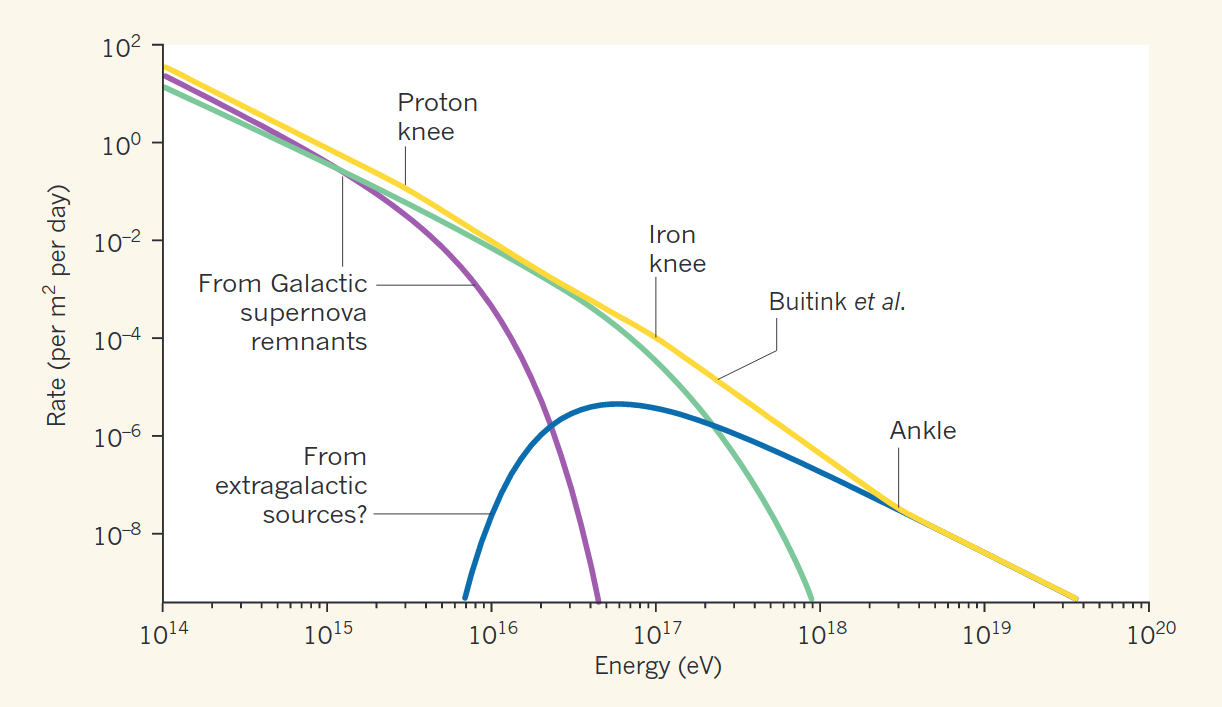
\includegraphics[width=\textwidth]{figure/andrew_superposition.png}
    % 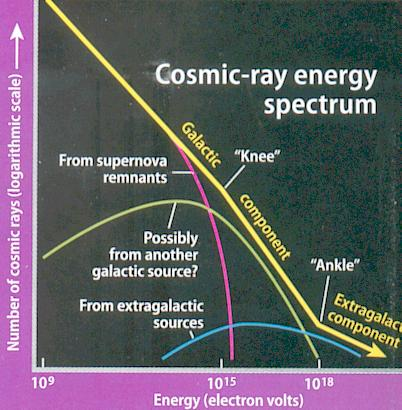
\includegraphics[height=0.7\textheight, width=0.9\textwidth]{CRFeature}
  \caption{
    CR spectrum
    (figure from \cite{taylor2016_crspectrumsuperposition})
  }
  \end{figure}
\end{frame}

%---- Intro objective (PAMELA & AMS) ---
\begin{frame}
\frametitle{Previous study}
\begin{itemize}
  \item In 2011, PAMELA claimed to discover a break in CR proton spectrum at around 300 GV. \citep{adriani2011pamela}
  \item In 2014, \textit{Fermi} LAT found some hint of this break though the results were inconclusive. \citep{FermiEarth14}
  \item In 2015, the AMS-02 comfirmed this break.
\end{itemize}
% In 2015, the AMS collaboration claims that there is a broken in cosmic ray proton spectrum around 336 GV.
\begin{figure}
  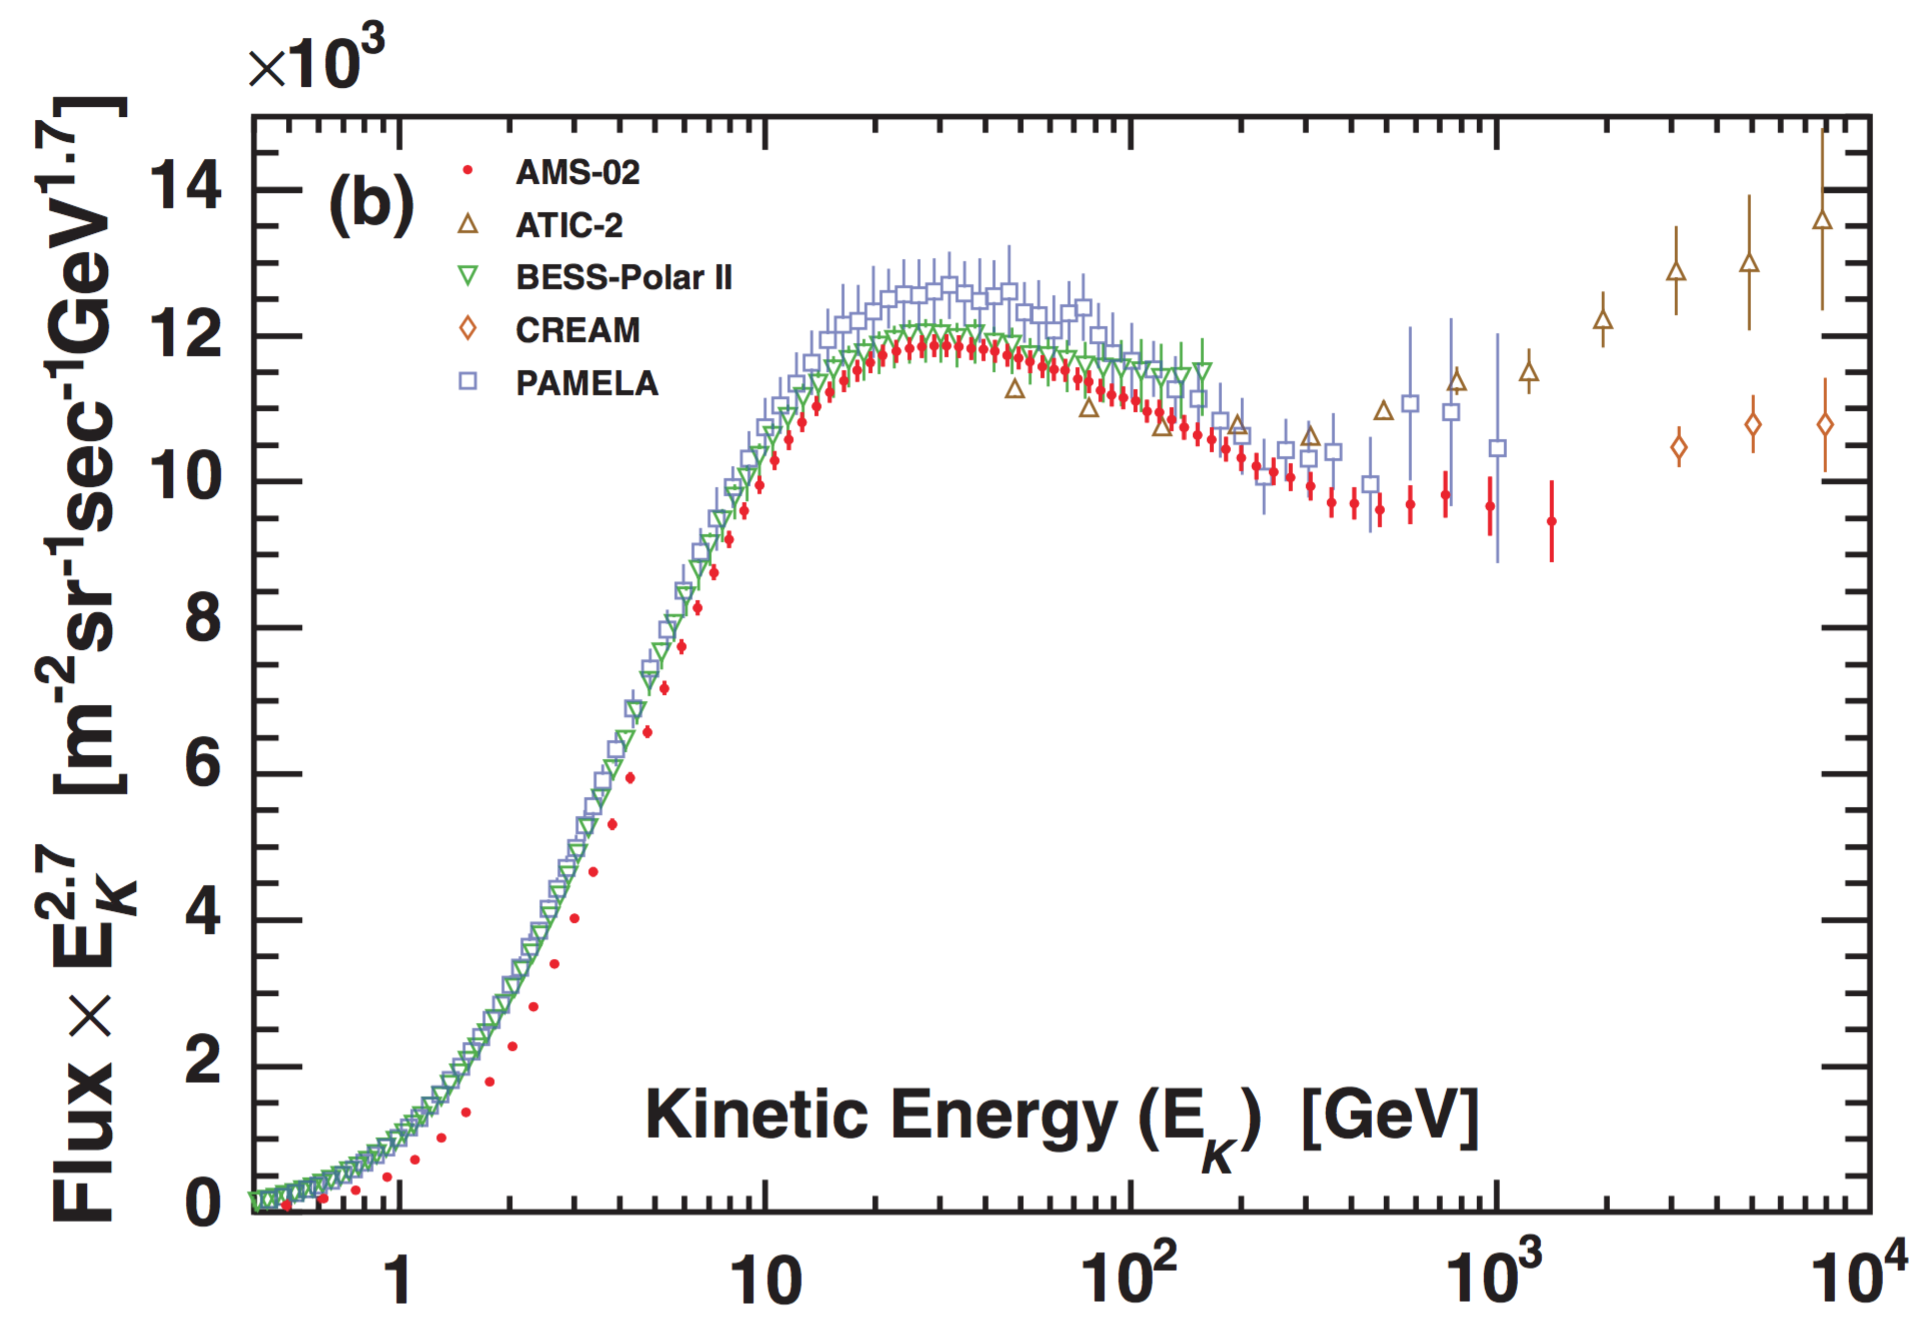
\includegraphics[width=0.55\textwidth]{proton_spectrum}
  \caption{CR proton flux from \cite{AMS02pr2015}}
\end{figure}
\end{frame}




%------ Production schematics --------------
% \subsection{Earth's limb $\gamma$-ray production}
\begin{frame}\frametitle{Earth's limb $\gamma$-ray production}
  \centering
  \begin{figure}[h!]
  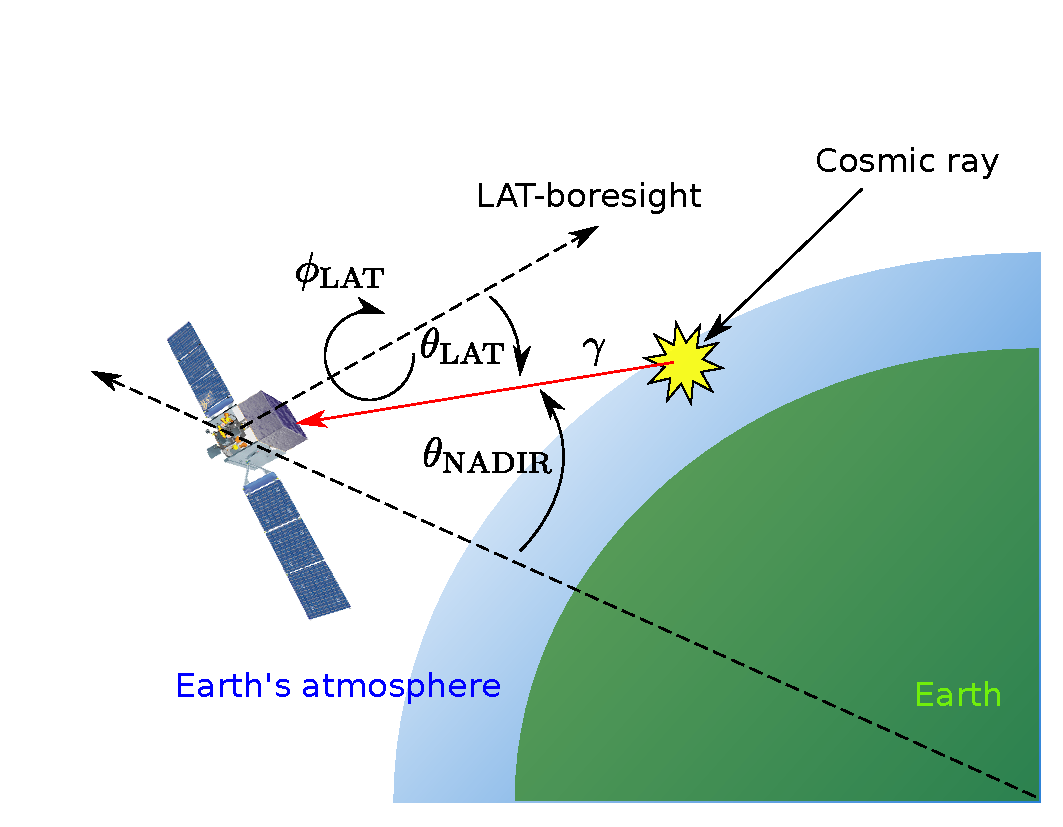
\includegraphics[width = 0.8\textwidth]{figure/for_lat_schematic/FermiLAT.pdf}
  \end{figure}
\end{frame}

%------------------------------------------------
%    3 ) Flux extraction
%------------------------------------------------
\section{Flux extraction}
%------------------------------------------------
%    3.2 ) Data set
%------------------------------------------------
\subsection{Data set}

\begin{frame}
\frametitle{Data selection}
\begin{itemize}
  \item P8R2\_ULTRACLEANVETO\_V6 data from 07/08/2008 to 17/10/2017 ($\sim$9 years) %Use P8R2\_ULTRACLEANVETO\_V6 data which collect only photon
  \item Photon energy range from 10 GeV up to 1 TeV
  \item $\theta_{\text{NADIR}}$ $\in$ 68.4$^\circ$  - 70$^\circ$
  (Thin-target $\gamma$-ray emission from the Earth's limb)
  \item $\theta_{\text{LAT}} < 70^\circ$
\end{itemize}
\end{frame}

%------------------------------------------------
%    3.3 ) Flux calculation
%------------------------------------------------
\subsection{Flux calculation}
%--- How to calculate flux ---
\begin{frame}
\frametitle{Flux calculation method}
\begin{enumerate}
  \item Analyze 50 bins in energy with equal logarithmic
  spacing between 10 GeV - 1 TeV  
  \item Create 2D histogram count maps from photon
  data for each energy bin
  \item Create 2D histogram exposure maps
  (effective area $\times$ livetime) from spacecraft data
  for each energy bin
  \item Calculate the Earth's $\gamma$-ray flux using the count and exposure maps by
  \begin{equation*}
    \textbf{Flux}(E_i) =  \frac{dN}{dE}(E_i) = \left(\sum_{\rm pixel} \frac{\text{Count}_i}{\text{Exposure}_i}\right) \frac{1}{\Delta\Omega\Delta E}
    \label{eq:def_flux}
  \end{equation*}
  % \item Create 2D histograms for 50 bins of $\gamma$-ray energy spectrum
  % \item Select photon data and fill in the 2D histograms
  % \item Calculate exposure maps which include the effective area and livetime of the LAT as it observed the Earth
  % \begin{equation}
  %   \textbf{Flux}(E_i) =  \frac{dN}{dE}(E_i) = \left(\int \frac{\text{Cnt}_i}{\text{Exp}_i}\right) \frac{1}{d(\Omega)dE_i}
  %   \label{eq:def_flux}
  % \end{equation}
\end{enumerate}
where $\Delta \Omega$ is the solid angle size of the
Earth's limb region, $\Delta E$ is the energy bin width,
and $i$ is the i$^{th}$ energy bin.
% where $\delta\Omega$ is the solid angle of the Earth's limb region and $\delta E$ is the energy bin width
\end{frame}
% %--- cntmap ---


%--- transform exposure map ---
\subsection{Exposure calculation}

\begin{frame}\frametitle{Coordinate Transformations}
\tikzstyle{block} = [rectangle, draw, fill=blue!10, 
text width=5em, text centered, rounded corners, minimum height=2em]
\tikzstyle{line} = [draw,thick, -latex']

\begin{columns}
  \column{0.5\textwidth}
    \begin{figure}[!h]
      \centering
      \begin{tikzpicture}[node distance = 6em, auto]
          \node [block, fill=black!10] (sp) {Local Zenith (zn)};
          \node [block, below of = sp] (eq) {Equatorial (eq)};
          \node [block, below of = eq] (p) {Detector Plane Boresight (p)};
          
          \draw[thick, <->] (eq) to node {$T_{\text{eq}, \text{p}}(\delta^\text{x}_\text{p}, \alpha^\text{x}_\text{p}, \delta^\text{z}_\text{p}, \alpha^\text{z}_\text{p}$)} (p);
          \draw[thick, <->] (eq) to node {$T_{\text{eq}, \text{zn}}(\delta_\text{zn}, \alpha_\text{zn})$} (sp);
      \end{tikzpicture}
      \caption{Three reference frames}
    \end{figure}

  \column{0.5\textwidth}
    where 
    \begin{itemize}
    \item \textbf{Local zenith (zn)}: x-axis points to LAT's zenith,
    z-axis to Earth's North
    \item \textbf{Equatorial (eq)}: z-axis points along Earth's rotation axis,
    x-axis towards the vernal equinox
    \item \textbf{Detector plane bore sight (p)}: z-axis points along LAT's boresight,
    x-axis along one solar panel
    \end{itemize}
\end{columns}
\end{frame}

%----- ZN-EQ -----------
\begin{frame}\frametitle{Coordinate Transformation: zn-eq}
  \begin{columns}
    \column{0.5\textwidth}
    \begin{figure}[h!]
      \centering
      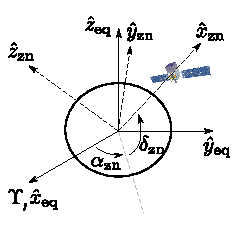
\includegraphics[width=0.8\textwidth]{figure/fig_coordinate/coord_eq_sp_v3.pdf}
    \end{figure}

    \column{0.5\textwidth}
      Transformation matrix could be extracted from the relation
      \begin{equation*}
        \hat{r}_\text{zn} \equiv T_{\text{eq}\rightarrow\text{zn}} (\delta_\text{zn}, \alpha_\text{zn}) \hat{r}_\text{eq}
      \end{equation*}
  \end{columns}

Write a unit vector of orbiting spacecraft on the basis of equatorial coordinate
\begin{equation*}
  \begin{split}
  \hat{x}_\text{zn} &= \cos\delta_\text{zn}\cos\alpha_\text{zn}\hat{x}_\text{eq} + \cos\delta_\text{zn}\sin\alpha_\text{zn}\hat{y}_\text{eq} + \sin\delta_\text{zn}\hat{z}_\text{eq}\\
  \hat{z}_\text{zn} &= - \sin\delta_\text{zn}\cos\alpha_\text{zn}\hat{x}_\text{eq} - \sin\delta_\text{zn}\sin\alpha_\text{zn}\hat{y}_\text{eq} + \cos\delta_\text{zn}\hat{z}_\text{eq} \\
  \hat{y}_\text{zn} &= \hat{z}_\text{zn} \times \hat{x}_\text{zn}.
  \end{split}
  \label{eq:tf_eq_sp}
\end{equation*}
\end{frame}

% \begin{frame}\frametitle{Coordinate Transformation: zn-eq}
%   \begin{figure}[h!]
%     \centering
%     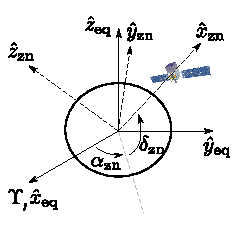
\includegraphics[width=0.5\textwidth]{figure/fig_coordinate/coord_eq_sp_v3.pdf}
%     \caption{Coordinate transformation between local zenith (zn) and equatorial (eq) coordinates}
%   \end{figure}
% \end{frame}

% \begin{frame}\frametitle{Coordinate Transformations: zn-eq}
% Write a unit vector of orbiting spacecraft on the basis of equatorial coordinate
% \begin{equation}
%   \begin{split}
%   \hat{x}_\text{zn} &= \cos\delta_\text{zn}\cos\alpha_\text{zn}\hat{x}_\text{eq} + \cos\delta_\text{zn}\sin\alpha_\text{zn}\hat{y}_\text{eq} + \sin\delta_\text{zn}\hat{z}_\text{eq}\\
%   \hat{z}_\text{zn} &= - \sin\delta_\text{zn}\cos\alpha_\text{zn}\hat{x}_\text{eq} - \sin\delta_\text{zn}\sin\alpha_\text{zn}\hat{y}_\text{eq} + \cos\delta_\text{zn}\hat{z}_\text{eq} \\
%   \hat{y}_\text{zn} &= \hat{z}_\text{zn} \times \hat{x}_\text{zn}.
%   \end{split}
%   \label{eq:tf_eq_sp}
% \end{equation}

% Transformation matrix could be extracted from the relation
% \begin{equation}
%   \hat{r}_\text{zn} \equiv T_{\text{eq}\rightarrow\text{zn}} (\delta_\text{zn}, \alpha_\text{zn}) \hat{r}_\text{eq}
% \end{equation}
% \end{frame}

%----- P-EQ -----------
\begin{frame}\frametitle{Coordinate Transformation: p-eq}
  \begin{columns}
    \column{0.5\textwidth}
    \begin{figure}[h!]
      \centering
      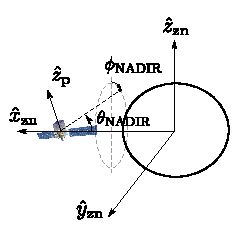
\includegraphics[width=0.9\textwidth]{figure/fig_coordinate/coord_eq_p_v3.pdf}
    \end{figure}

    \column{0.55\textwidth}
      Transformation matrix is defined as
      \begin{equation*}
        \hat{r}_\text{p} \equiv T_{\text{eq}\rightarrow\text{p}} (\delta^\text{x}_\text{p}, \alpha^\text{x}_\text{p}, \delta^\text{z}_\text{p}, \alpha^\text{z}_\text{p}) \hat{r}_\text{eq}
        \label{eq:rep_tf_eq_p}
      \end{equation*}

      Then 
      \begin{equation*}
      \begin{split}
        \hat{r}_\text{zn} & (\theta_\text{NADIR}, \phi_\text{NADIR}) \equiv -\cos\theta_\text{NADIR}\hat{x}_\text{zn}\\
        & + \sin\theta_\text{NADIR}\cos\phi_\text{NADIR}\hat{z}_\text{zn}\\
        & + \sin\theta_\text{NADIR}\sin\phi_\text{NADIR}\hat{y}_\text{zn}
      \end{split}
      \end{equation*}

  \end{columns}

\begin{equation*}
  \begin{split}
  \hat{x}_\text{p} &= \cos\delta^\text{x}_\text{p}\cos\alpha^\text{x}_\text{p}\hat{x}_\text{eq} + \cos\delta^\text{x}_\text{p}\sin\alpha^\text{x}_\text{p}\hat{y}_\text{eq} + \sin\delta^\text{x}_\text{zn}\hat{z}_\text{eq}\\
  \hat{z}_\text{p} &= \cos\delta^\text{z}_\text{p}\cos\alpha^\text{z}_\text{p}\hat{x}_\text{eq} + \cos\delta^\text{z}_\text{p}\sin\alpha^\text{z}_\text{p}\hat{y}_\text{eq} + \sin\delta^\text{z}_\text{zn}\hat{z}_\text{eq}\\
  \hat{y}_\text{p} &= \hat{z}_\text{p} \times \hat{x}_\text{p}
  \end{split}
  \label{eq:tf_eq_p}
\end{equation*}
\end{frame}


% \begin{frame}\frametitle{Coordinate Transformation: p-eq}
%   \begin{figure}[h!]
%     \centering
%     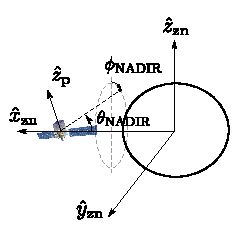
\includegraphics[width=0.5\textwidth]{figure/fig_coordinate/coord_eq_p_v3.pdf}
%     \caption{Coordinate transformation between LAT plane boresight and local zenith coordinates}
%   \end{figure}
% \end{frame}

% \begin{frame}\frametitle{Coordinate Transformations: p-eq}
% \begin{equation}
%   \begin{split}
%   \hat{x}_\text{p} &= \cos\delta^\text{x}_\text{p}\cos\alpha^\text{x}_\text{p}\hat{x}_\text{eq} + \cos\delta^\text{x}_\text{p}\sin\alpha^\text{x}_\text{p}\hat{y}_\text{eq} + \sin\delta^\text{x}_\text{zn}\hat{z}_\text{eq}\\
%   \hat{z}_\text{p} &= \cos\delta^\text{z}_\text{p}\cos\alpha^\text{z}_\text{p}\hat{x}_\text{eq} + \cos\delta^\text{z}_\text{p}\sin\alpha^\text{z}_\text{p}\hat{y}_\text{eq} + \sin\delta^\text{z}_\text{zn}\hat{z}_\text{eq}\\
%   \hat{y}_\text{p} &= \hat{z}_\text{p} \times \hat{x}_\text{p}
%   \end{split}
%   \label{eq:tf_eq_p}
% \end{equation}

% \begin{equation}
%   \hat{r}_\text{p} \equiv T_{\text{eq}\rightarrow\text{p}} (\delta^\text{x}_\text{p}, \alpha^\text{x}_\text{p}, \delta^\text{z}_\text{p}, \alpha^\text{z}_\text{p}) \hat{r}_\text{eq}
%   \label{eq:rep_tf_eq_p}
% \end{equation}
% \end{frame}

%----- Summarize TF -----------
\begin{frame}\frametitle{Coordinate Transformation: Compact formula}
  \begin{figure}[h!]
    \centering
    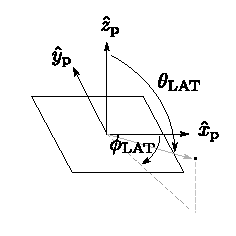
\includegraphics[width=0.45\textwidth]{figure/fig_coordinate/coord_plane_v2.pdf}
  \end{figure}
  \begin{equation*}
  \begin{split}
    \hat{r}_\text{p} (\theta_\text{NADIR}, \phi_\text{NADIR}) = & T_{\text{eq}\rightarrow\text{p}} (\delta^\text{x}_\text{p}, \alpha^\text{x}_\text{p}, \delta^\text{z}_\text{p}, \alpha^\text{z}_\text{p}) \\
    & \times \left[T_{\text{eq}\rightarrow\text{zn}} (\delta_\text{zn}, \alpha_\text{zn})\right]^{-1} \hat{r}_\text{zn} (\theta_\text{NADIR}, \phi_\text{NADIR})
  \end{split}
  \end{equation*}
\end{frame}

%----- Parallel computing -----------
\begin{frame}\frametitle{Exposure calculation: procedures}
Given a spacecraft log file (FT2) where it contains a row-like 
of the telescope status. The calculation steps are
  \begin{itemize}
    \item Pick a row in FT2
    \item Compute transformation matrices
    \item Mapping each nadir cell to the plane of detector
    \item Computes exposure time $\times$ effective area
  \end{itemize}

Then iterate this process for all records from a selected timeframe.
\end{frame}


\begin{frame}\frametitle{Exposure calculation: parallel computing}
  \begin{figure}[h!]
    \centering
    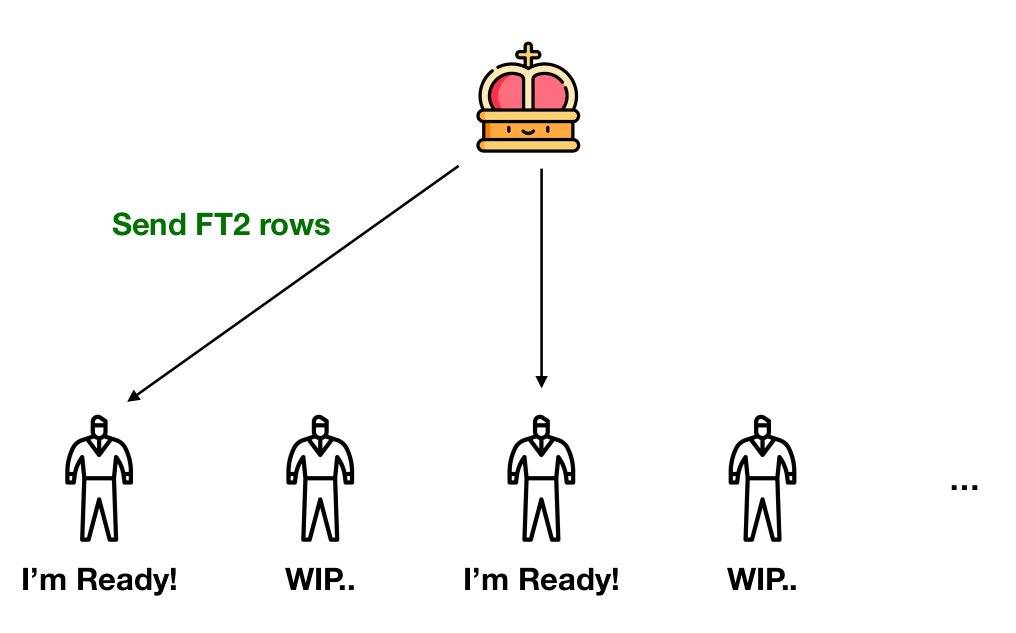
\includegraphics[width=0.9\textwidth]{figure/ms3.png}
    \caption{
      Demonstrations of Master-Slave technique. WIP stands for working in progress.
    }
  \end{figure}
\end{frame}


%------------------------------------------------
%    4 ) Methodology
%------------------------------------------------
\section{Analysis}

% ------- poewr law in rigidity -------------
\subsection{Power-law spectrum}

\begin{frame}
  \frametitle{Power-law models (in rigidity)}
  We use 2 models of CR proton to fit the Earth's $\gamma$-ray data: \\
  \textbf{Single power law (SPL)}
  \begin{equation*}
  \frac{dN}{dR} = R_0R^{-\Gamma}
  \end{equation*}
  \textbf{Broken power law (BPL)}
  \begin{equation*}
  \frac{dN}{dR}=
    \begin{cases}
      R_0R^{-\Gamma_1}\ :\ E < E_{\text{Break}}\\
      R_0[R(E_{\text{Break}})]^{\Gamma_2-\Gamma_1}R^{-\Gamma_2}\ :\ E \ge E_{\text{Break}}
    \end{cases}
  \end{equation*}
  Rigidity is defined by $R\equiv P/q$ where $P$ is the momentum and $q$ is the absolute value of the charge (in unit of proton charge) of a particle
\end{frame}
%------------------------------------------------
%    4.1 ) K&O model
%------------------------------------------------
\subsection[$pp\rightarrow\gamma$ model]{Proton-proton $\rightarrow$ $\gamma$ model}
\begin{frame}
\frametitle{Kachelriess and Ostapchenko model}
This model can compute the $\gamma$-ray spectrum from a broad and smooth power-law spectrum of CR protons
% Is the model which can compute spectrum of $\gamma$-ray from a known incident proton
\begin{equation*}
  % \small
  \frac{dN_{\gamma}}{dE_{\gamma}} \propto\sum_{E'_i}\left[\frac{E'_i}{E_{\gamma}}\Delta(\ln E'_i) \right]\left[ f_{pp}\textcolor{red}{\frac{dN_p}{dE'_i}}\left\{ 1+\textcolor{olivegreen}{\frac{\sigma_{\text{HeN}}}{\sigma{pN}}}\left(\textcolor{red}{\frac{dN_p}{dR}}\right)^{-1} \textcolor{blue}{\frac{dN_{\text{He}}}{dR}} \frac{dR_{\text{He}}}{dR_p}  \right\}\right]
\end{equation*}
\begin{itemize}
  \item Red color terms are for \textcolor{red}{incident proton spectrum}
  \item \textcolor{blue}{Blue color term is the He spectrum from AMS-02 (2015)}
  \item $f_{pp}\equiv E_\gamma(d\sigma^{pp\rightarrow\gamma}/dE_\gamma)$ is the interaction cross section table in the K\&O model \citep{K&Omodel}
  \item The cross-section ratio \textcolor{olivegreen}{$\sigma_{\text{HeN}}/\sigma_{pN}$} at high energy ($>$ 10GeV) is roughly constant ($\approx 1.6$) \citep{WAtwater}
\end{itemize}

\end{frame}
%------------------------------------------------
%    4.1 Optimization
%------------------------------------------------
\subsection{Optimization}
\begin{frame}
\frametitle{Poisson likelihood function}
% On the previous slide, we want to find the incident proton. \\
% Let define some loss function to compare model and measurement
% \begin{equation}
%   \mathcal{L} = \prod_{i=1}^{N} P_{\text{pois}}(n_{\text{i,model}}, n_{\text{i,measurement}})
% \end{equation}
We determine the incident proton spectrum that best fits the $\gamma$-ray masurement using the maximum likelihood (or minimum log likelihood) method

% For numerically convenient, redefined into logarithmic form
\begin{equation*}
  \log\mathcal{L} \equiv \sum_{i=1}^{\textcolor{blue}{N}} -\log P_{\text{pois}}(n_{\text{i,model}}, n_{\text{i,measurement}})
\end{equation*}
% This part is the hard work of computer to find best incident cosmic ray proton that match the
% spectrum from measurement.
where $P_{\text{pois}}$ is the Poisson probability of measuring $n_{\text{i,measurement}}$ counts when the model predicts $n_{\text{i,model}}$ counts for \textit{\textcolor{blue}{N}} energy bins

\end{frame}

\begin{frame}\frametitle{Fitting algorithm: Particle Swarm Optimization}
\begin{itemize}
  \item Randomly initiate many particles in a given range of the parameter space
  \item Check global and local best particle from a defined profit function
  \item The rest of them move toward the global and local particles
  \item Iterate the process until most of them yield nearly the same profit
\end{itemize}
\begin{figure}
\begin{columns}
  \begin{column}{0.34\textwidth}
    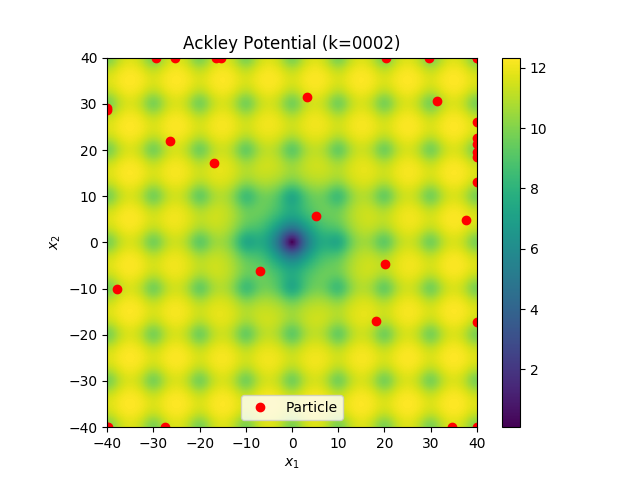
\includegraphics[width=\columnwidth]{figure/particle_swarm0002}
  \end{column}
  \begin{column}{0.34\textwidth}
  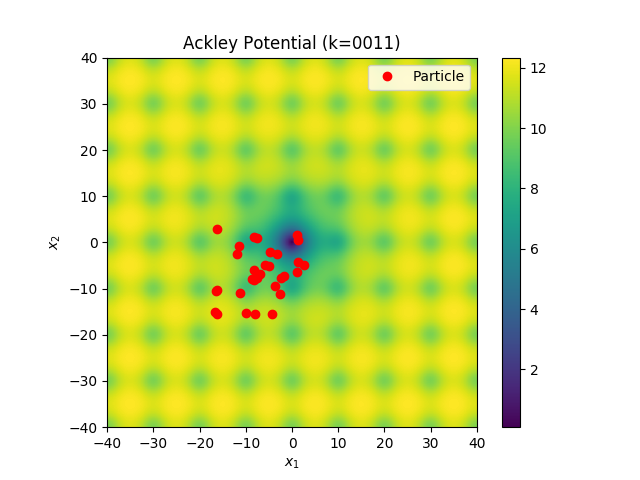
\includegraphics[width=\columnwidth]{figure/particle_swarm0011}
  \end{column}
  \begin{column}{0.34\textwidth}
    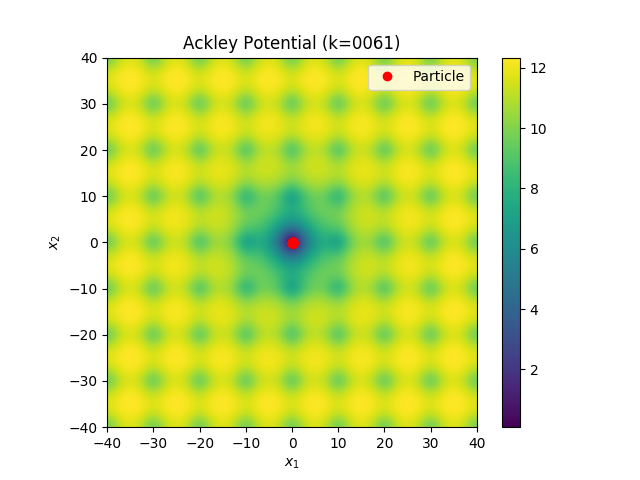
\includegraphics[width=\columnwidth]{figure/particle_swarm0061}
  \end{column}
\end{columns}
\caption{Example of particles in parameter space of Ackley potential}
\end{figure}
\end{frame}


\begin{frame}\frametitle{Particle Swarm Optimization}
For every iteration $k$, particle $i$ move with velocity $v^i_k$ where
\begin{equation*}
  v^i_{k+1} = \omega v^i_k + c^br^b_k[b^i_k-x^i_k] + c^Br^B_k[B^i_k-x^i_k]
\end{equation*}
Update the new state of particle $i$ with
\begin{equation*}
  x^i_{k+1} = x^i_k + v^i_{k+1}
\end{equation*}
where
\begin{itemize}
  \item $x^i_k$ represent variable that particle $i$ hold
  \item $b$ and $B$ are best local and global parameter sets along the optimization process
  \item Set $\omega = 0.2$, $c^b = 0.2$ and $c^B = 0.3$
\end{itemize}
The iteration process would stop when standard deviation of fitness over any partilcle less than 0.1
\end{frame}

% %-- Flow chart ---%
%   % Define block styles
%   \tikzstyle{decision} = [diamond, draw, fill=red!10, 
%   text width=2em, text badly centered, node distance=2.5cm, inner sep=0pt]
%   \tikzstyle{block} = [rectangle, draw, fill=blue!10, 
%   text width=5em, text centered, rounded corners, minimum height=2em]
%   \tikzstyle{longblock} = [rectangle, draw, fill=blue!10, 
%   text width=10em, text centered, rounded corners, minimum height=4em]
%   \tikzstyle{line} = [draw,thick, -latex']
%   \tikzstyle{cloud} = [draw, ellipse,fill=red!20, node distance=3cm,
%   minimum height=4em]

% \begin{frame}\frametitle{Algorithm}

% \begin{figure}[!h]
% \centering
% \begin{tikzpicture}[node distance = 6em, auto]
%     \node [block, fill=black!10] (powerlaw) {powerlaw spectrum of proton in rigidity};
%     \node [block, right of = powerlaw, node distance = 12em] (model) {$\gamma$-ray spectrum from model};
%     \node [block, right of = model] (measurement) {$\gamma$-ray spectrum from measurement};
%     \node [block, below left of = measurement, node distance = 8em] (pois) {Poisson likelihood function};
%     \node [block, below of = powerlaw] (varyPar) {Apply gradient to parameters $\gamma$, $R_0$};
%     \node [decision, below of = varyPar, fill = blue!10] (bestfit) {Best fit?};
%     \node [block, right of = bestfit, node distance = 10em, fill = red!10] (return) {Return best fit parameters};

%     \path [line] (powerlaw) -- node [anchor=south] {K\&O model} (model);
%     \path [line] (model) -- (pois);
%     \path [line] (measurement) -- (pois);
%     \path [line] (pois) -- (bestfit);
%     \path [line] (bestfit) -- node [anchor=east] {No} (varyPar);
%     \path [line] (varyPar) -- (powerlaw);
%     \path [line] (bestfit) -- node [anchor=north] {Yes} (return);
% \end{tikzpicture}
% \caption{Flow chart of optimization process}
% \end{figure}

% \end{frame}

%------------------------------------------------
%    4.3 ) Results
%------------------------------------------------
\section{Results and Discussion}
\subsection{$\gamma$-ray flux}

%--- flxmap ---
\begin{frame}
  \frametitle{Flux maps}
  \begin{figure}[h!]
  \begin{tikzpicture}
  \node (0,0) {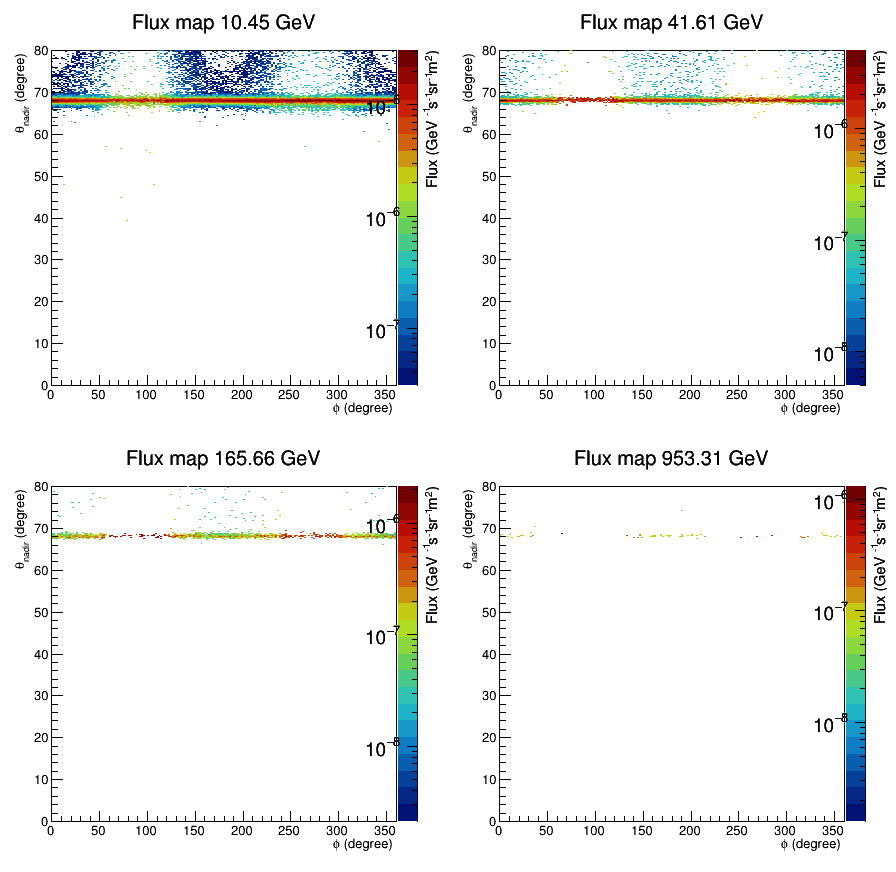
\includegraphics[height=0.9\textheight]{figure/cartesian_flxmaps_v2}};
  % \node [opacity=0.2] (0,0) {\rotatebox{45}{\scalebox{3.5}{\textcolor{red}{preliminary}}}};
  \end{tikzpicture}
  \end{figure}
\end{frame}

\begin{frame}
  \frametitle{Flux maps}
  \begin{figure}[h!]
  \begin{tikzpicture}
  \node (0,0) {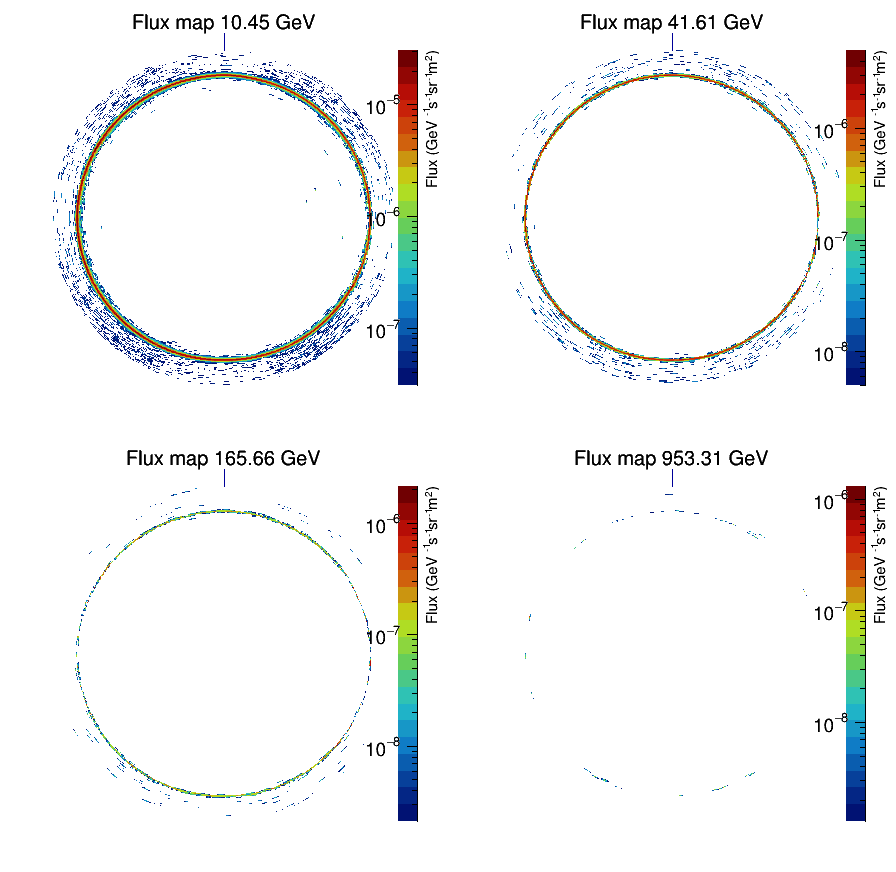
\includegraphics[height=0.9\textheight]{figure/polar_flxmaps_v2}};
  % \node [opacity=0.2] (0,0) {\rotatebox{45}{\scalebox{3.5}{\textcolor{red}{preliminary}}}};
  \end{tikzpicture}
  \end{figure}
\end{frame}
  
  

%--- got spectrum ---
\begin{frame}
  \frametitle{Earth's limb $\gamma$-ray spectrum from measurement}
  \begin{figure}[h!]
    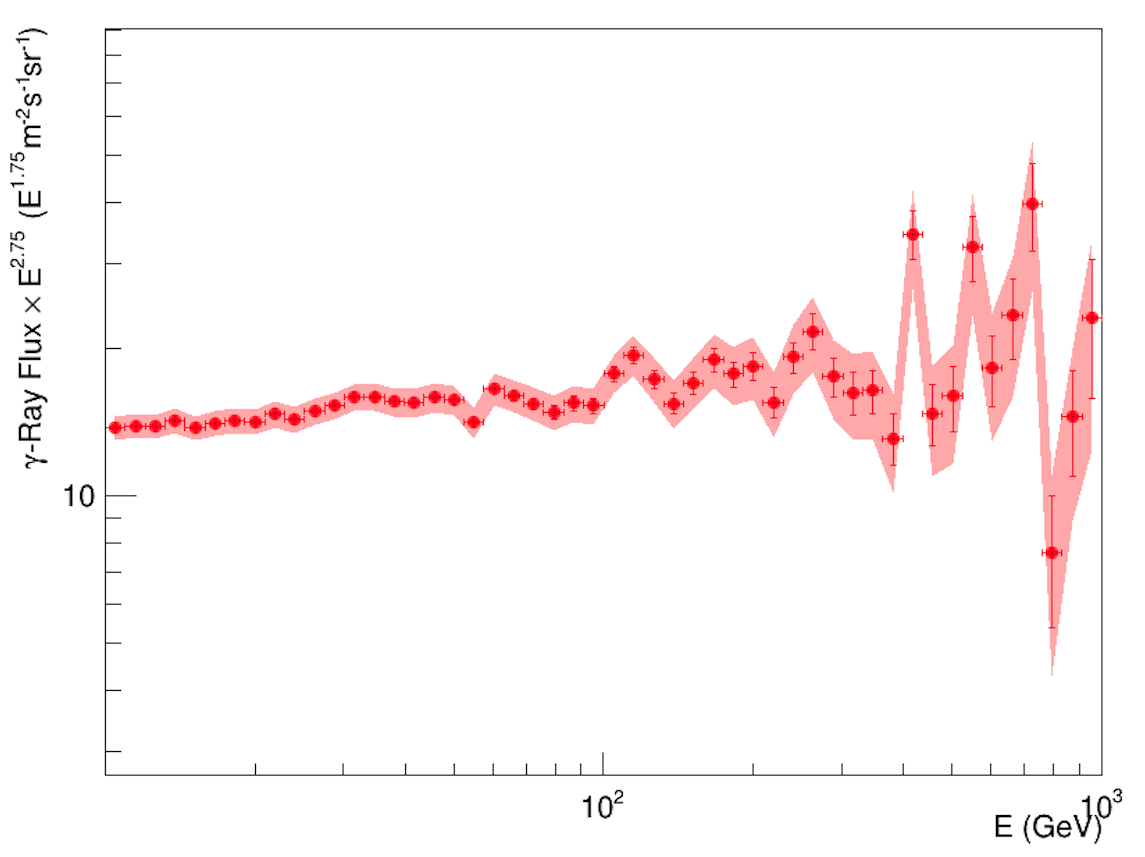
\includegraphics[width=0.65\textwidth]{figure/gamma_spectrum}
  \end{figure}
  \small
  Error bars show statistical uncertainties and
  red bands show total (statistical + systematic) uncertainties.
  Systematic error is 5\% from 10 GeV to 100 GeV
  and $5\% + 10\%\times (\log_{10}(E/\text{MeV})-5)$ above 100 GeV.
\end{frame}

% --- table results
\subsection{Optimized results}
\begin{frame}
\frametitle{Results}
\begin{table}
\begin{tabular}{l | c | c | c}
  Best fits & $\Gamma_1$ & $\Gamma_2$ & $E_{\text{Break}}$ (GeV) \\
  \hline \hline
  SPL & 2.70 & - & -  \\
  BPL & 2.86 & 2.63 & 333
\end{tabular}
\caption{Optimization results.}
\end{table}

From the hypothesis testing of BPL versus SPL, it yields
a confidence level at $1.38\sigma$ (92\%).

\end{frame}

% --- graph gamma ray
\begin{frame}
\frametitle{Earth's limb $\gamma$-ray spectra from best-fit models}

\begin{figure}
  \begin{tikzpicture}
  \node (0,0) {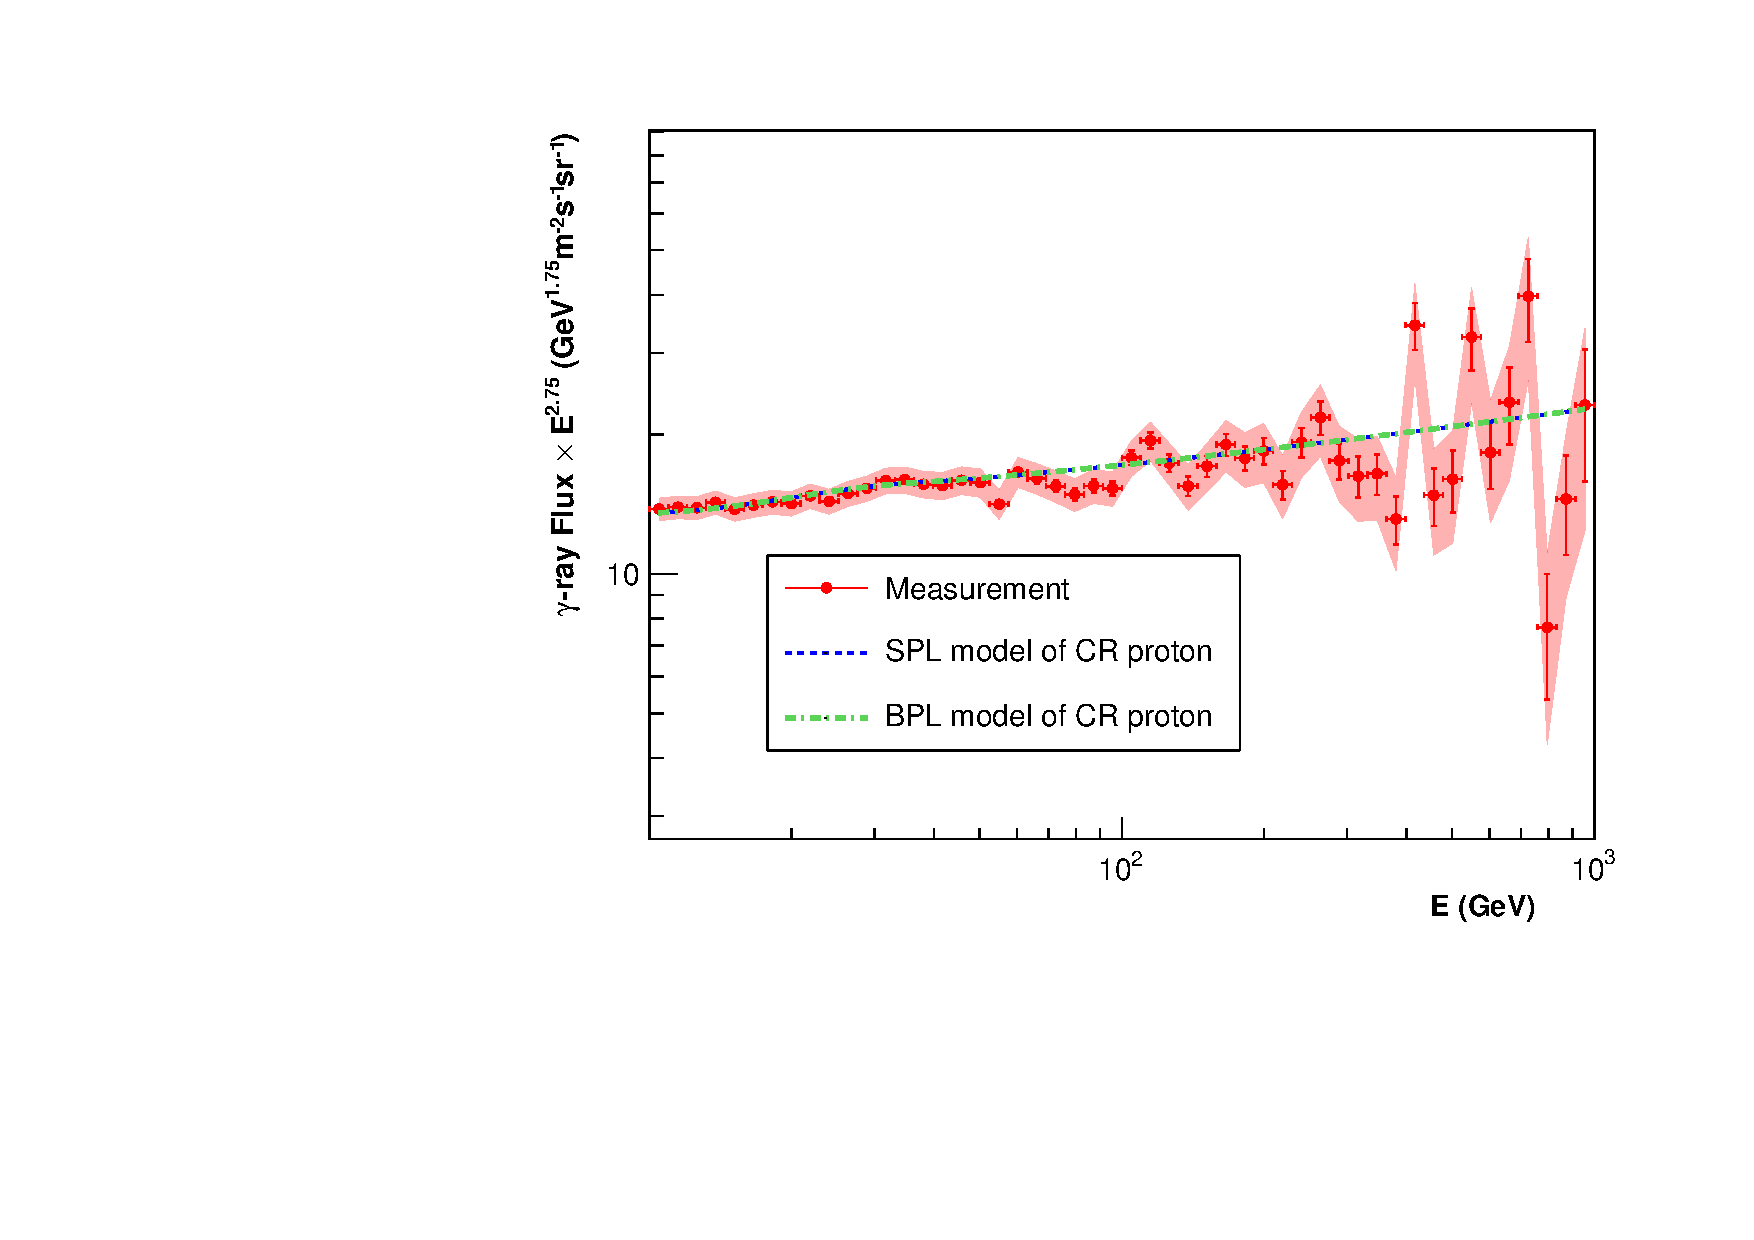
\includegraphics[width=0.85\textwidth]{figure/fitted_result}};
  % \node [opacity=0.2] (0,0) {\rotatebox{45}{\scalebox{2.5}{\textcolor{red}{preliminary}}}};
  % \node [opacity=1.0] at (2.7,-2.75) {\tiny E (GeV)};
  \end{tikzpicture}
\end{figure}


\end{frame}
% --- spectrum proton
\begin{frame}
  \frametitle{Proton spectrum}
  
  \begin{figure}[h!]
  \begin{tikzpicture}
  \node (0,0) {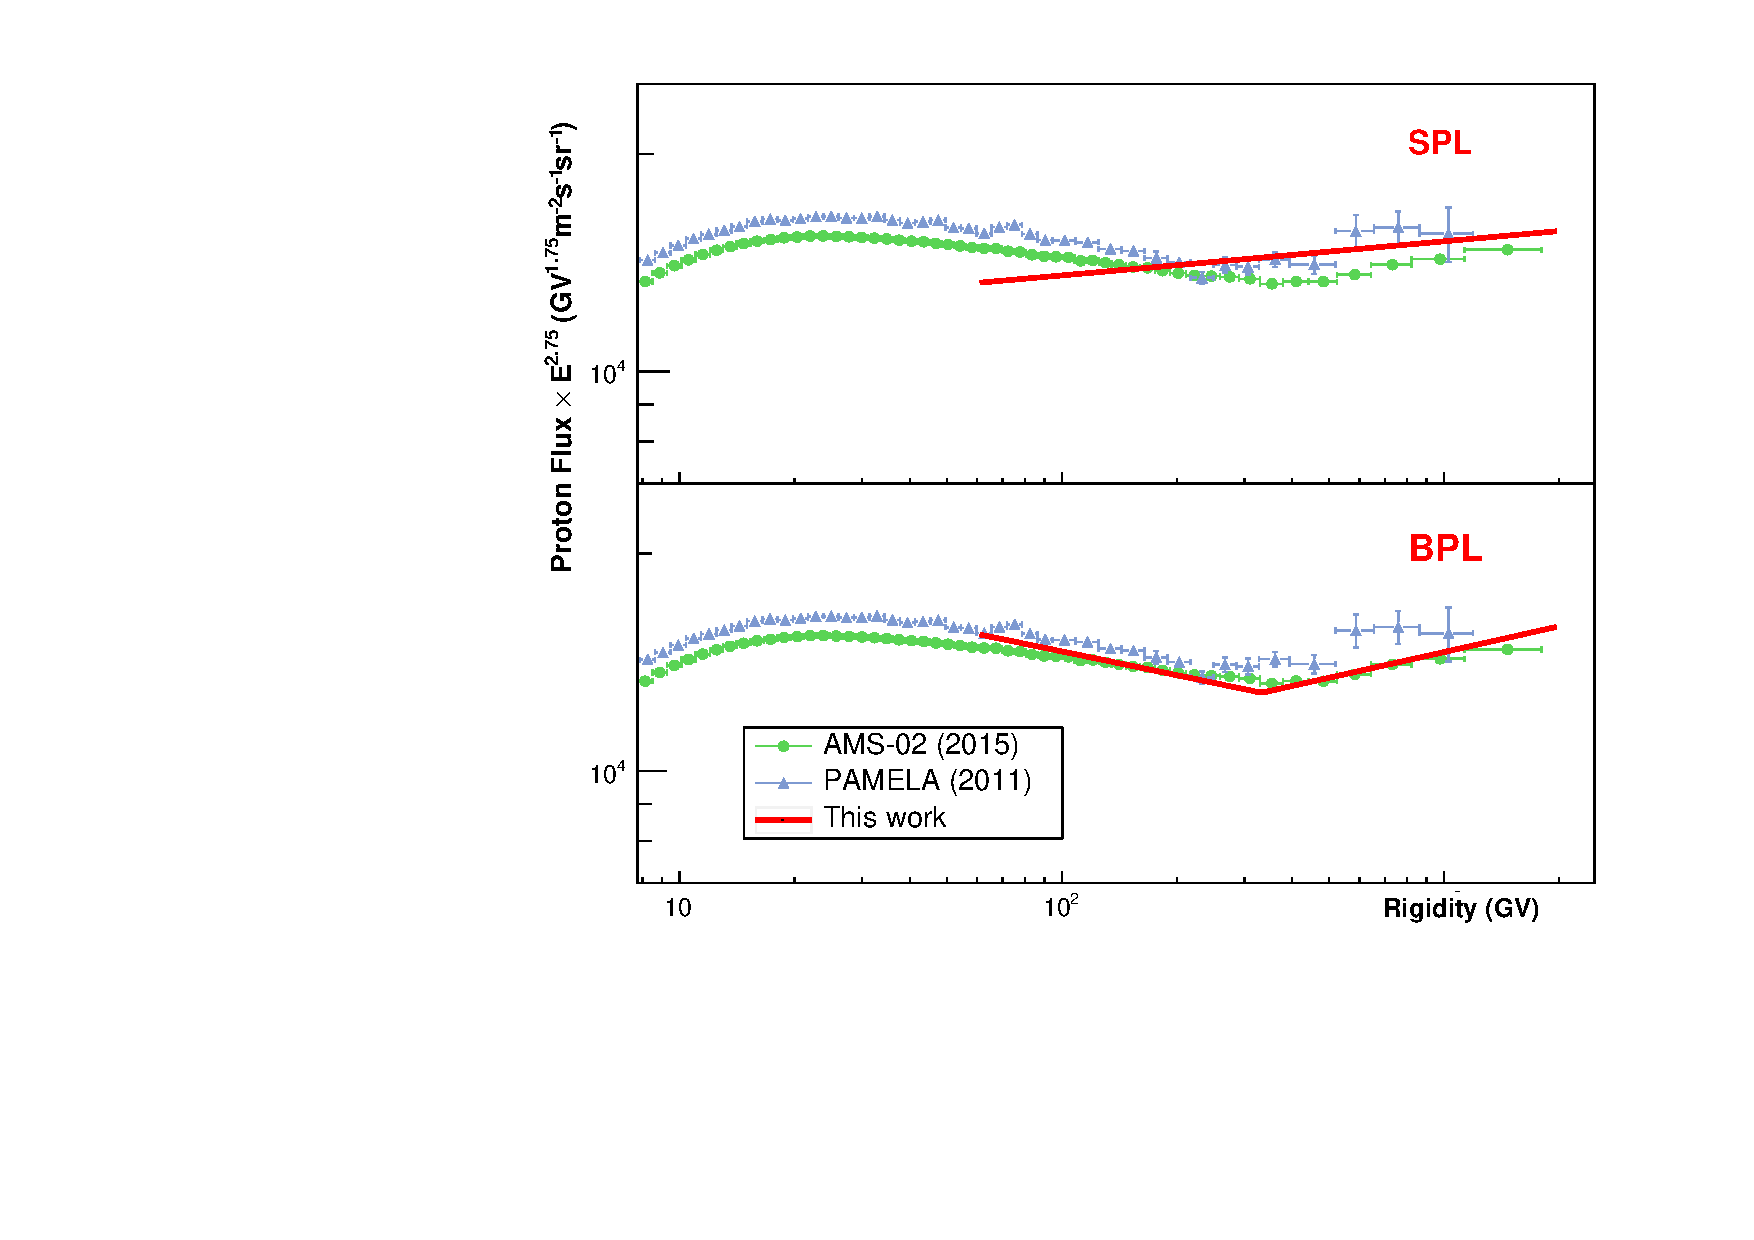
\includegraphics[width=0.8\textwidth]{ProtonSpectrumModelMeasurement}};
  % \node [opacity=0.2] (0,0) {\rotatebox{45}{\scalebox{2.5}{\textcolor{red}{preliminary}}}};
  \end{tikzpicture}
  \end{figure}
\tiny The normalization of this work is fitted AMS-02 data  
\end{frame}
%------------------------------------------------
%    4.4 ) Monte carlo Simulation
%------------------------------------------------
% \subsection{Monte Carlo simlation}
% %----- How to deal with this ?
% \begin{frame}
% \frametitle{Error determination}
% \textbf{Statictical error (Random error)}
% \begin{enumerate}
%   \item Get back to raw count and
%   \textcolor{blue}{random new count in each energy bin by Poisson random function}
%   \item Recalculate proton spectrum
%   \item Optimize it and store the parameter that we got
%   \item do it over thoundsand time and fill in histogram to interpret error by saying sigma of gaussian function
% \end{enumerate}
% \textbf{Total error (take into account instrument)}
% \begin{enumerate}
%   \item Get back to raw count and
%   \textcolor{blue}{random new count in each energy bin by Poisson random function}
%   \item \textcolor{blue}{Random value we got again by systematic error (Apparatus)}
%   \item Recalculate proton spectrum
%   \item Optimize it and store the parameter that we got
%   \item do it over thoundsand time and fill in histogram to interpret error by saying sigma of gaussian function
% \end{enumerate}
% \end{frame}

% %----- SPL ------
% \begin{frame}
% \frametitle{Single power law (SPL)}

% \begin{figure}[h!]
% \begin{tikzpicture}
% \node (0,0) {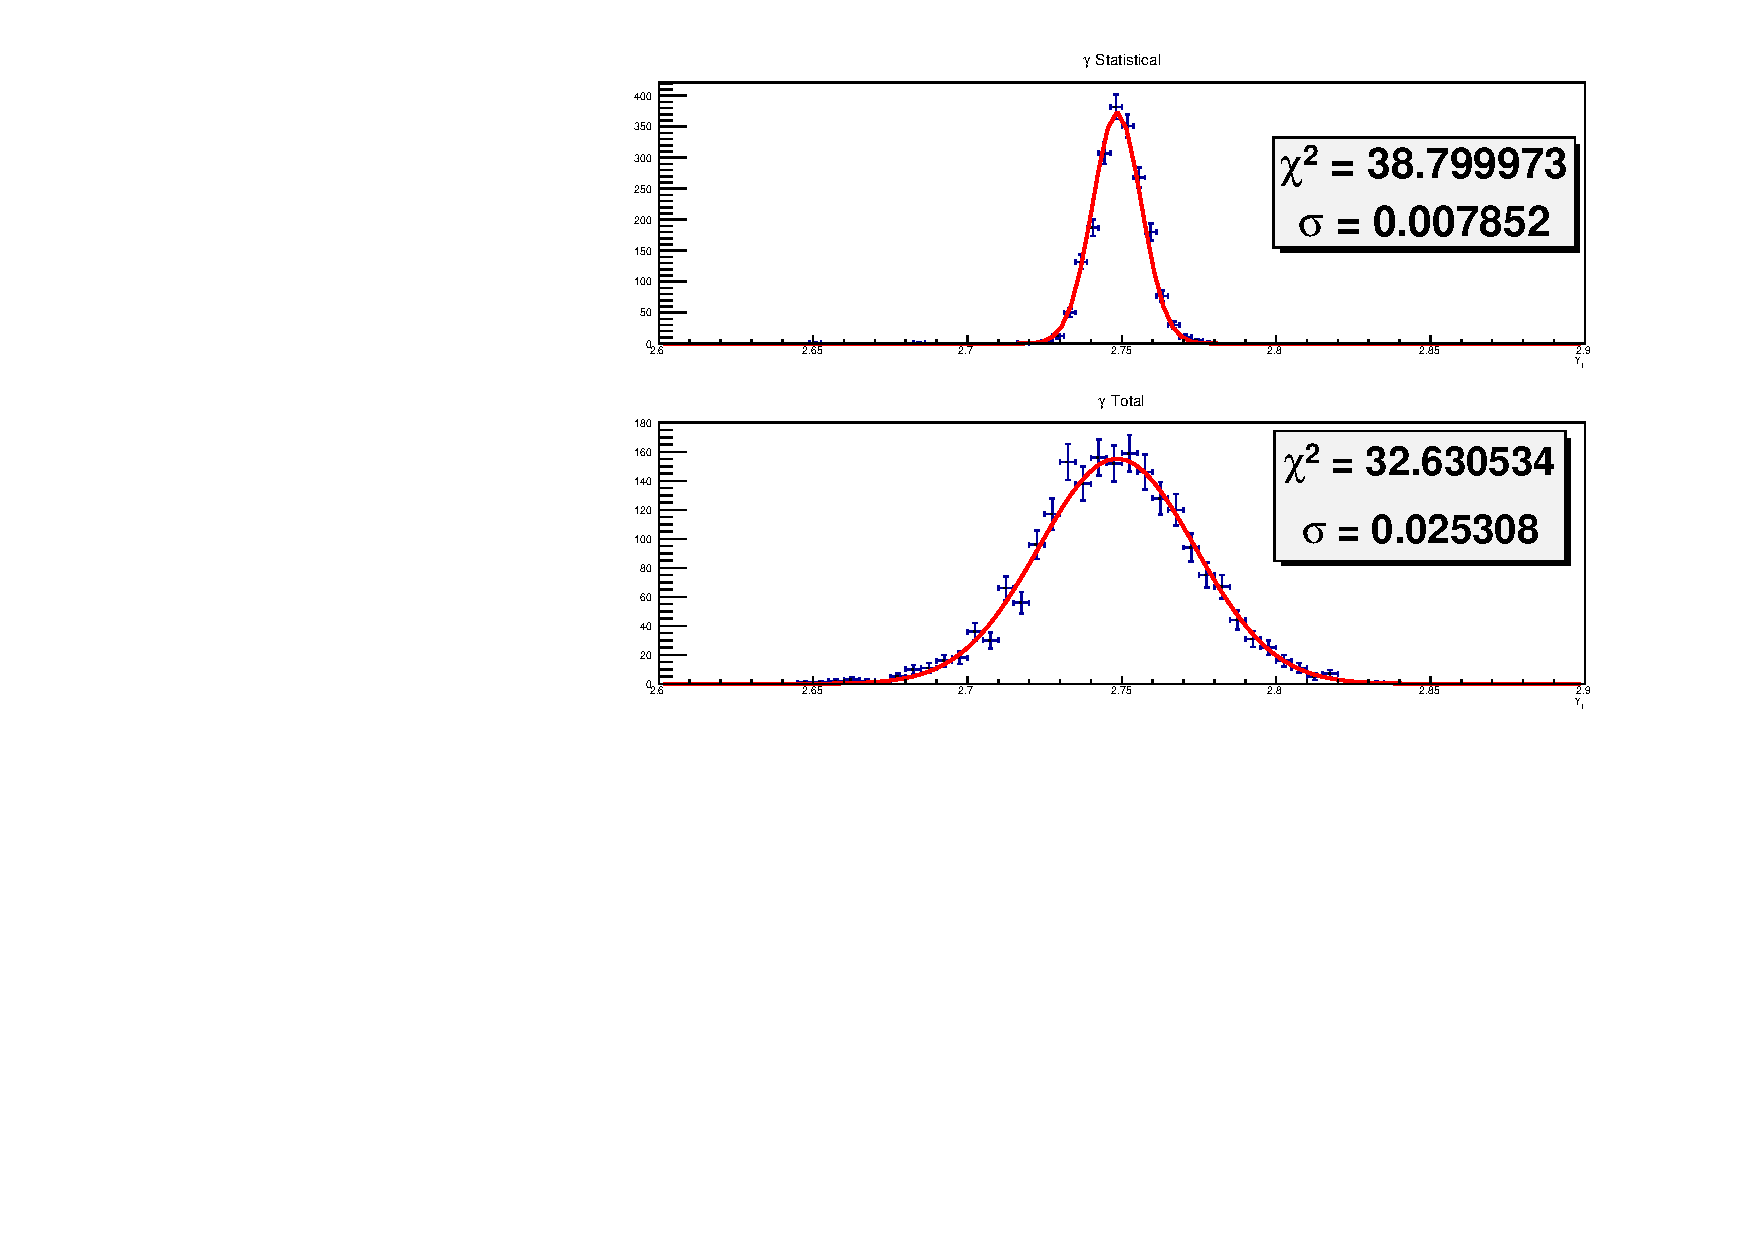
\includegraphics[width=0.8\textwidth]{SPL_Sim}};
% \node [opacity=0.2] (0,0) {\rotatebox{45}{\scalebox{3.0}{\textcolor{red}{preliminary}}}};
% \end{tikzpicture}
% \end{figure}

% \end{frame}
% %------ BPL ------
% \begin{frame}
% \frametitle{Broken power law (BPL)}

% %\begin{figure}[h!]
% %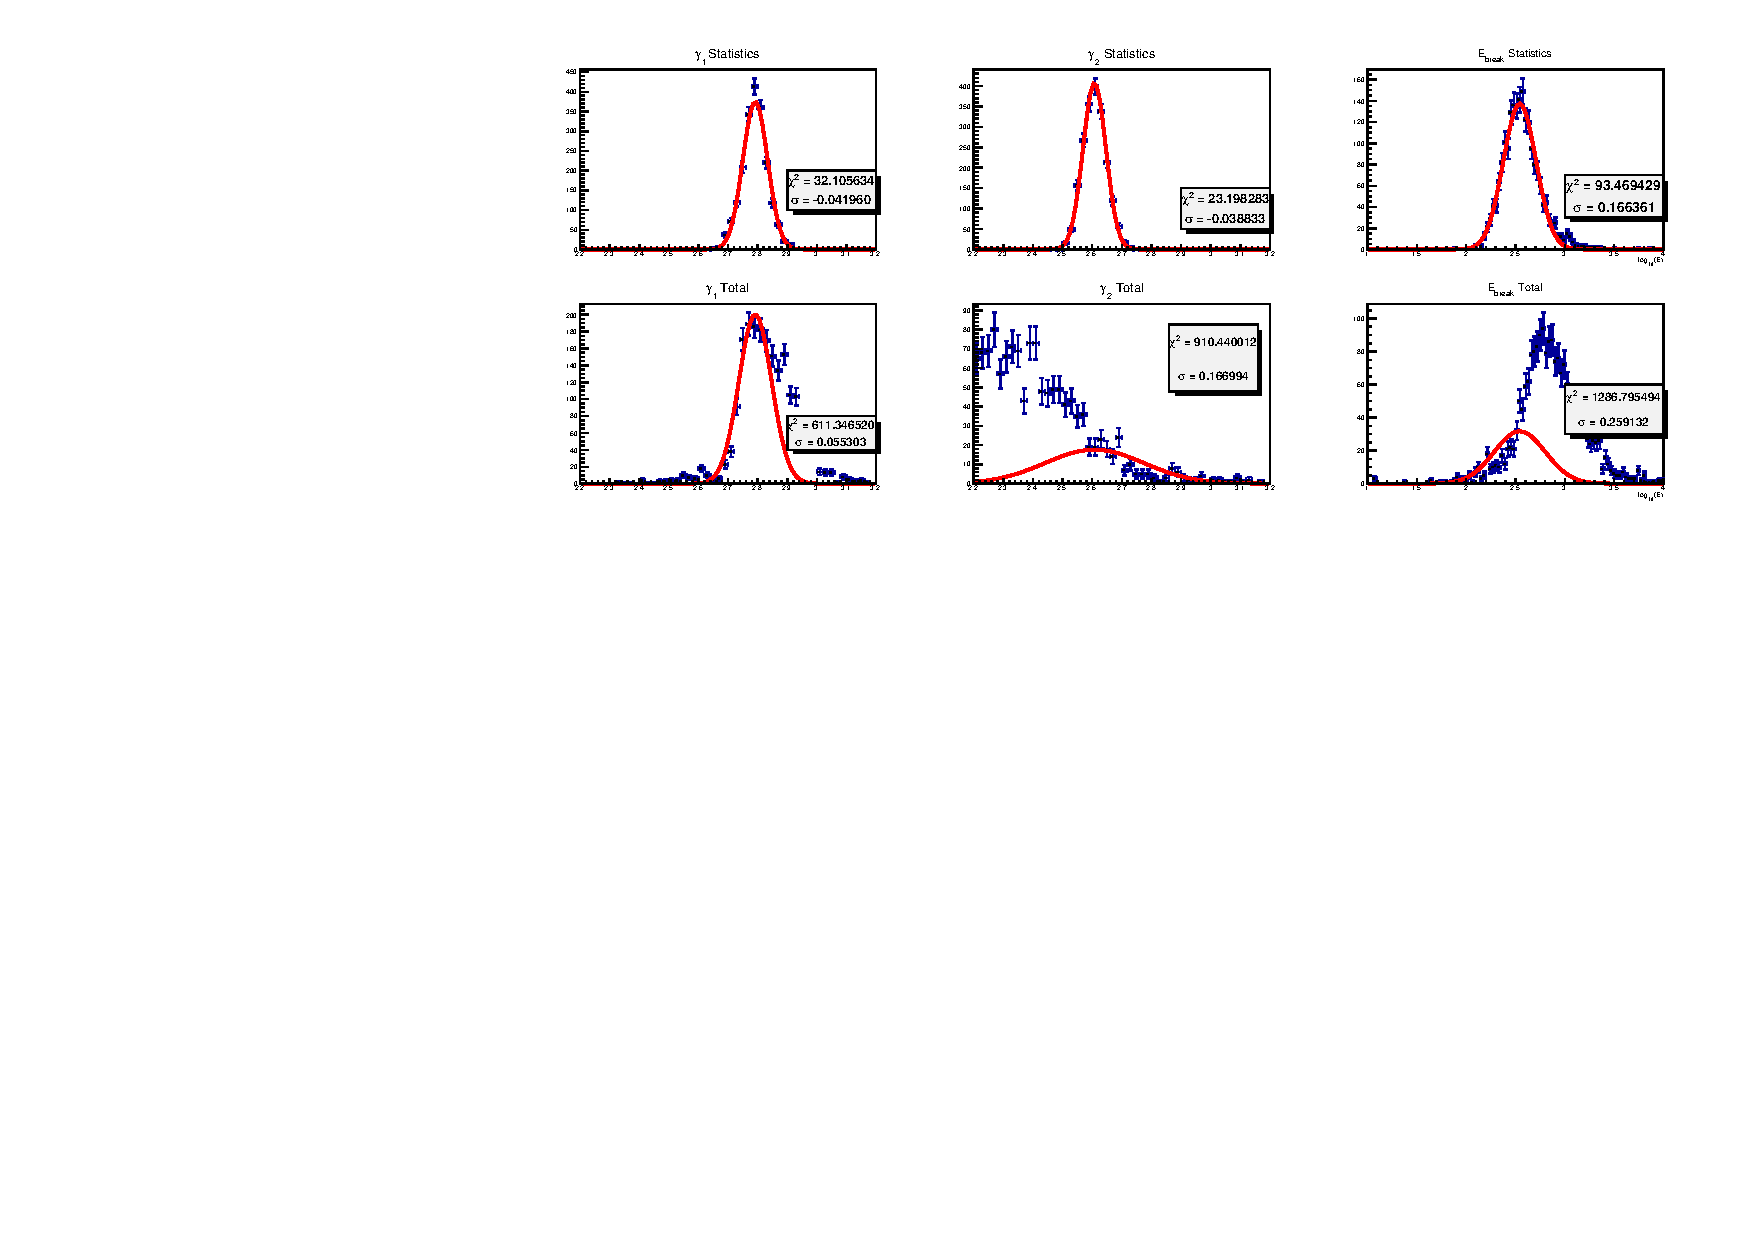
\includegraphics[width = \textwidth]{BPL_Sim}
% %\end{figure}

% \begin{figure}[h!]
% \begin{tikzpicture}
% \node (0,0) {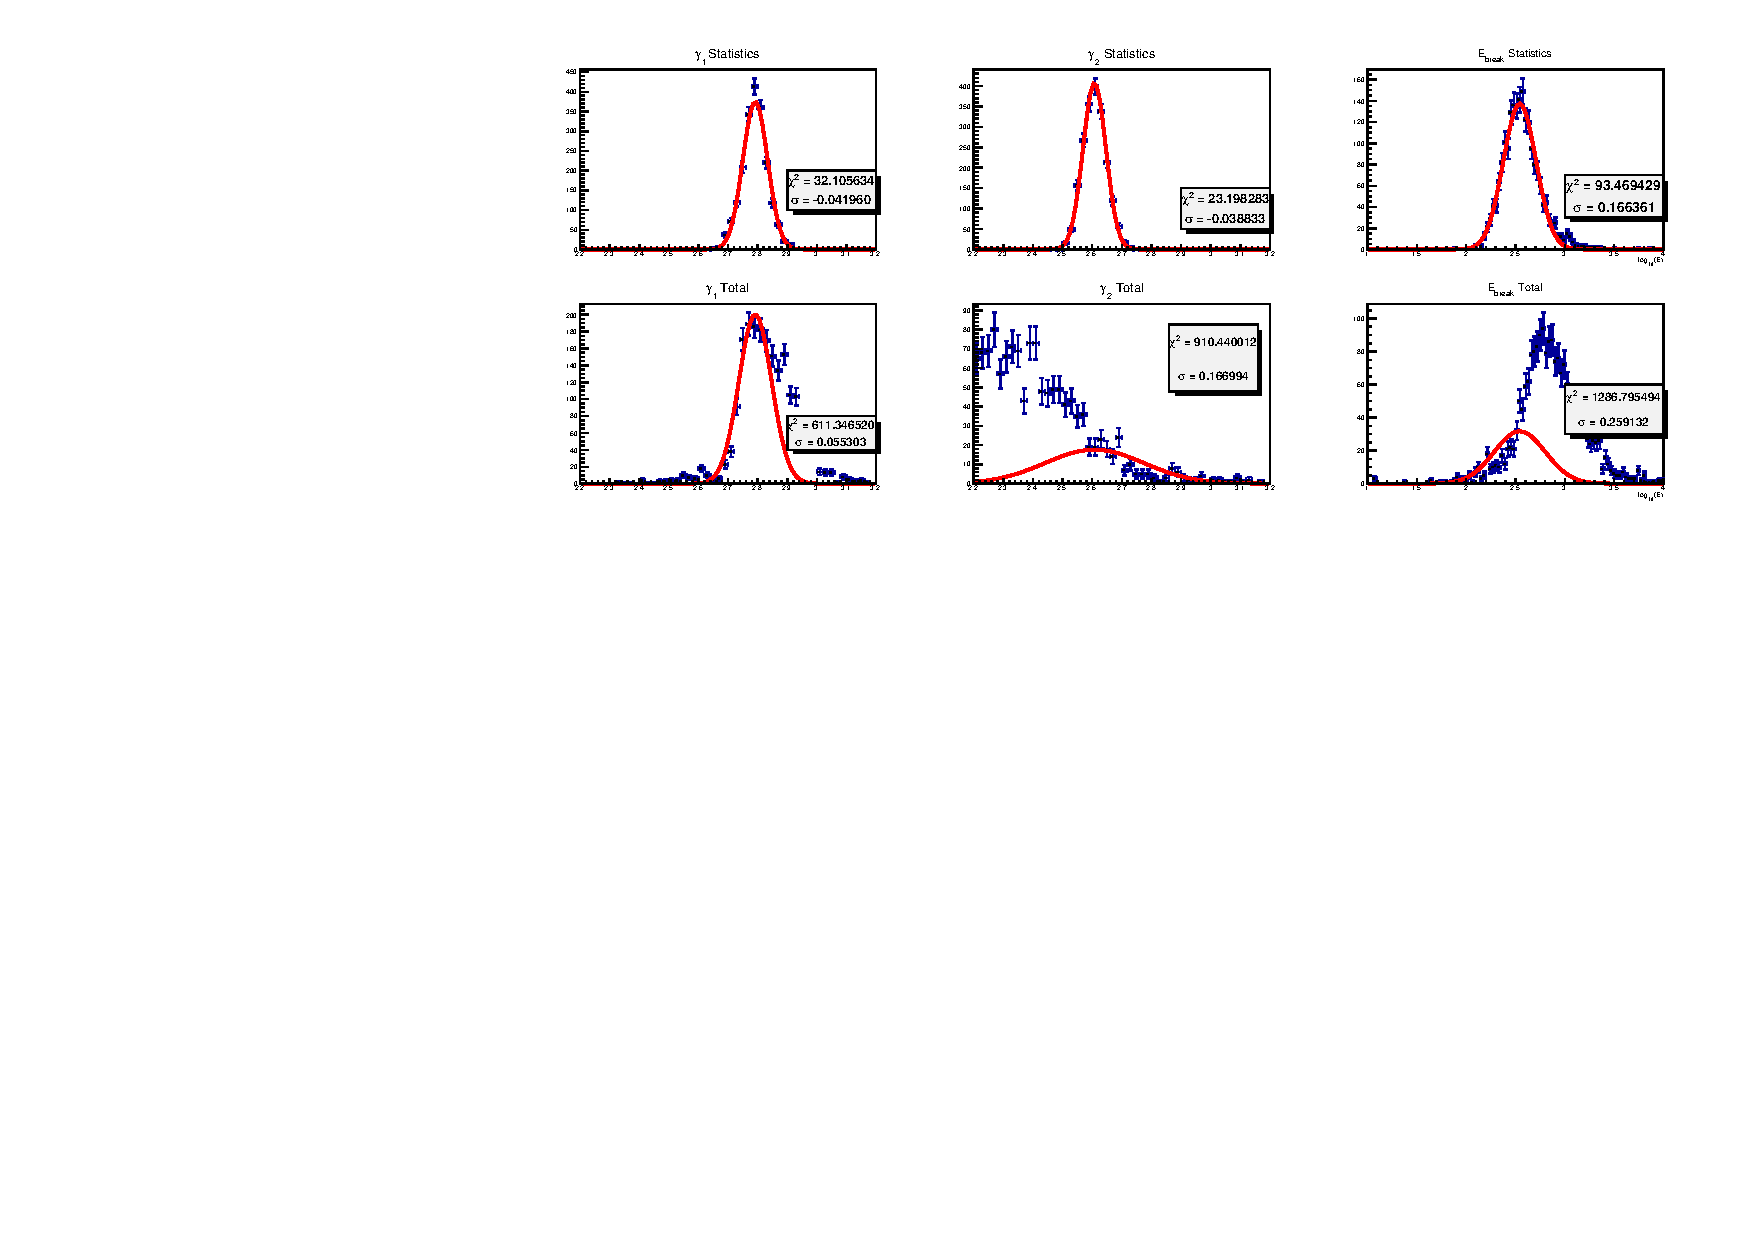
\includegraphics[width=\textwidth]{BPL_Sim}};
% \node [opacity=0.2] (0,0) {\rotatebox{25}{\scalebox{3.5}{\textcolor{red}{preliminary}}}};
% \end{tikzpicture}
% \end{figure}

% \end{frame}
% %------------------------------------------------
% %   4 )  To do list
% %------------------------------------------------
% \section{To do list}
% \begin{frame}
% \frametitle{To do}
% \begin{itemize}
% \item Problem of shifted value in BPL came from optimization algorithm because it stop in local minimum
% \item Extract new Flux due to technical problem (Still doubt.. might came from exposure map or photon selection)
% \item Fix bug in my log-likelihood function (Use count instread of flux)
% \item Resimulate data when I am done above stuff
% \end{itemize}
% \end{frame}

%------------------------------------------------
%   Conclusion
%------------------------------------------------
\section{Summary}
\begin{frame}
\frametitle{Summary}
\begin{itemize}
  \item Our best BPL fit indicates the spectral hardening of
  CR proton at $\sim$ 333 GV
  \item This breaking point is consistent with the direct measurement
  by AMS-02 at $\sim 336^{+66}_{-28}$ GV and the previous indirect measurement
  by Fermi LAT at $\sim$ 302 $\pm$ 62 GV
  \item The BPL model fits the measured Earth's $\gamma$-ray
  spectrum better than the SPL model does at the significance
  level of 1.38$\sigma$ (compared to 1.0$\sigma$ in previous
  LAT analysis)
  \item Though with more than 2x increase in the amount of data,
  the spectral break cannot be concluded exclusively by this work
  \item This indirect detection method may reach its limitation
  due to the systematic uncertainties
\end{itemize}

% \begin{itemize}
%   \item The results shows a consistency with direct measurement 
%   (AMS-02) where breaking point is $\sim$ 340 GV (ours 333 GV)
%   \item The significant level is 1.37$\sigma$ (previous work 1.0$\sigma$)
%   \item Put the weights on the indirect measurement approach
% \end{itemize}
\end{frame}


%------------------------------------------------


%------------------------------------------------
% \section{} % just empty section for not showing header on slide
\appendix

%------------------------------------------------
%    Reference
%------------------------------------------------
\begin{frame}
\frametitle{References}
\bibliographystyle{abbrvnat} % alpha abbrvnat
\tiny
\bibliography{mybib}

% [1] O. Adriani et al., Science 332, 69 (2011) \newline
% [2] M. Ackermann et al. (\textit{Fermi} LAT Collaboration), Phys. Rev. Lett. 112, 151103 (2015) \newline
% [3] Kachelriess $\&$ Ostapchenko, Phys. Rev. D 86 (2012) \newline
% [4] M. Aguilar et al. (AMS Collaboration), Phys. Rev. Lett. 115, 211101 (2015) \newline
% [5] M. Aguilar et al. (AMS Collaboration), Phys. Rev. Lett. 114, 171103 (2015) \newline
% [6] L. Lyons, Statistics for nuclear and particle physicists
\end{frame}

%------------------------------------------------
%    Acknowledgement
%------------------------------------------------
\begin{frame}\frametitle{Acknowledgement}
  \begin{itemize}
    \item Asst. Prof. Warit Mitthumsiri, Prof. David Ruffolo \\ Mahidol University, Thailand
    \item Dr. Francesca Spada \\ University of Pisa, Italy
    \item People in the Space Physics Laboratory at Mahidol University and the \textit{Fermi}-LAT research group at the University of Pisa
    \item Development and Promotion of Science and Technology Talents Project (DPST)
    \item Partially supported by the Thailand Science Research and Innovation (RTA6280002)
  \end{itemize}
\end{frame}

%------------------------------------------------
%    Back up slide
%------------------------------------------------

\begin{frame}
\Huge{\centerline{Backup slide}}
\end{frame}

% % ------- poewr law in rigidity -------------
% \begin{frame}
% \frametitle{Power law (in rigidity)}
% Typically, cosmic ray spectrum follow power law in rigidity as \\
% \textbf{Single power law (SPL)}
% \begin{equation}
% \frac{dN}{dR} = R_0R^{-\gamma}
% \end{equation}
% \textbf{Broken power law (BPL)}
% \begin{equation}
% \frac{dN}{dR}=
%   \begin{cases}
%     R_0R^{-\gamma_1}\ :\ E < E_{\text{Break}}\\
%     R_0[R(E_{\text{Break}})]^{\gamma_2-\gamma_1}R^{-\gamma_2}\ :\ E \ge E_{\text{Break}}
%   \end{cases}
% \end{equation}
% Note for someone who not famoliar with rigidity : it just defined by $R\equiv P/q$ when $P, q$ is a momentum and charge of particle
% \end{frame}
% ------- power law in Energy -------------
\begin{frame}
\frametitle{Power law in energy}
Converting the power law in rigidity to energy, we obtain
\textbf{Single power law (SPL)}
\begin{equation*}
\frac{dN}{dE} = N_0[E_k(E_k+2m_p)]^{-\gamma/2} \left(\frac{E_k+m_p}{\sqrt{E_k(E_k+2m_p)}}\right)
\end{equation*}
\textbf{Broken power law (BPL)}
\begin{equation*}
\frac{dN}{dE}=
  \begin{cases}
    N_0[E_k(E_k+2m_p)]^{-\gamma_1/2} \left(\frac{E_k+m_p}{\sqrt{E_k(E_k+2m_p)}}\right)\ :\ E < E_{\text{Break}}\\
    N_0[E_b(E_b+2m_p)]^{(\gamma_2-\gamma_1)/2}[E_k(E_k+2m_p)]^{-\gamma_2/2} \left(\frac{E_k+m_p}{\sqrt{E_k(E_k+2m_p)}}\right)\\ :\ E \ge E_{\text{Break}}
  \end{cases}
\end{equation*}
\end{frame}


%----------------------------------
% ---------  calculation map --------
%----------------------------------
%--- cntmap ---
\begin{frame}
\frametitle{Count map}
\begin{figure}[h!]
\begin{tikzpicture}
\node (0,0) {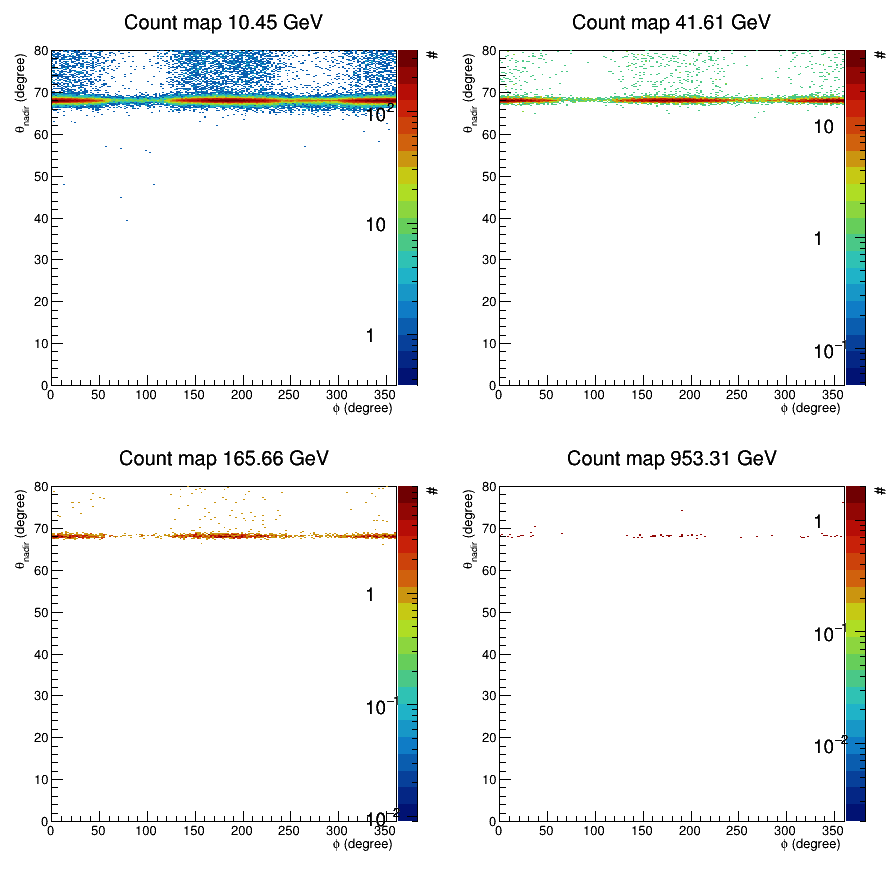
\includegraphics[height=0.9\textheight]{figure/cartesian_cntmaps_v2}};
% \node [opacity=0.2] (0,0) {\rotatebox{45}{\scalebox{3.5}{\textcolor{red}{preliminary}}}};
\end{tikzpicture}
\end{figure}
\end{frame}

\begin{frame}
\frametitle{Count maps}
\begin{figure}[h!]
\begin{tikzpicture}
\node (0,0) {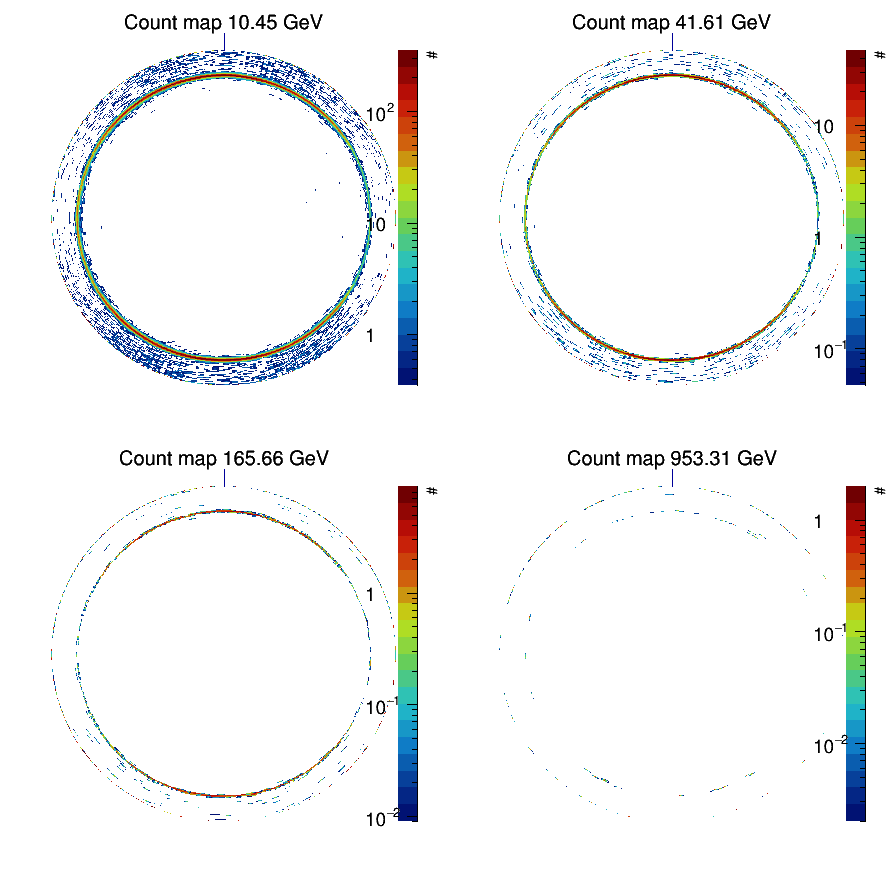
\includegraphics[height=0.9\textheight]{figure/polar_cntmaps_v2}};
% \node [opacity=0.2] (0,0) {\rotatebox{45}{\scalebox{3.5}{\textcolor{red}{preliminary}}}};
\end{tikzpicture}
\end{figure}
\end{frame}
%--- expmap ---
\begin{frame}
\frametitle{Exposure maps}
\begin{figure}[h!]
\begin{tikzpicture}
\node (0,0) {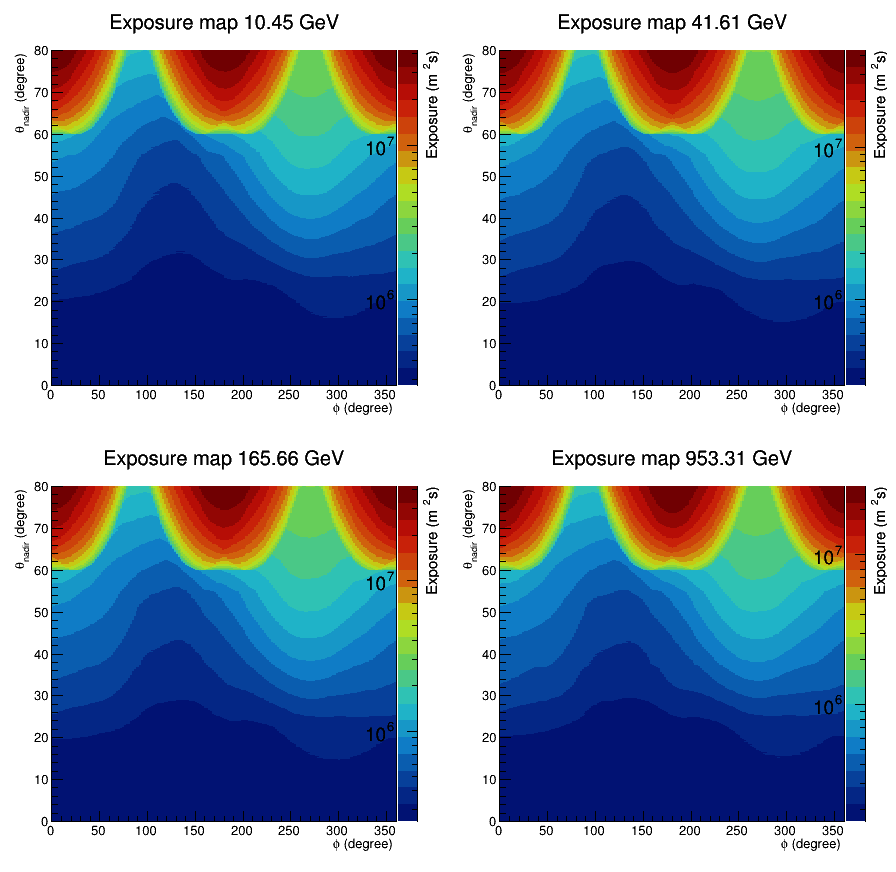
\includegraphics[height=0.9\textheight]{figure/cartesian_expmaps_v2}};
% \node [opacity=0.2] (0,0) {\rotatebox{45}{\scalebox{3.5}{\textcolor{red}{preliminary}}}};
\end{tikzpicture}
\end{figure}
\end{frame}

\begin{frame}
\frametitle{Exposure maps}
\begin{figure}[h!]
\begin{tikzpicture}
\node (0,0) {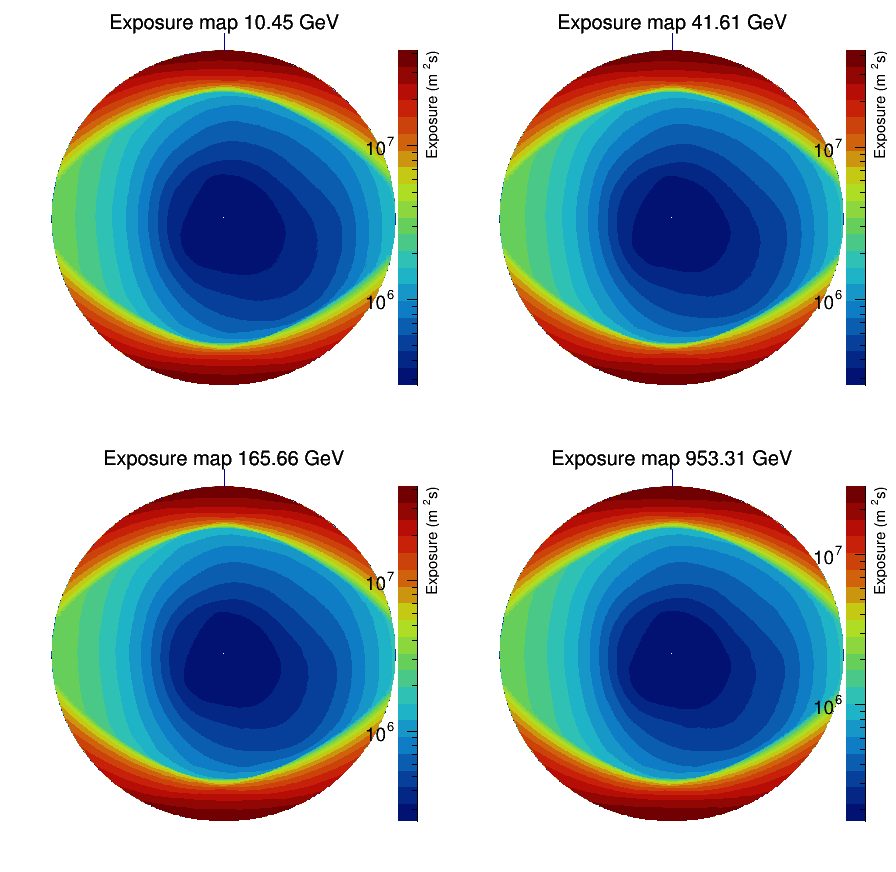
\includegraphics[height=0.9\textheight]{figure/polar_expmaps_v2}};
% \node [opacity=0.2] (0,0) {\rotatebox{45}{\scalebox{3.5}{\textcolor{red}{preliminary}}}};
\end{tikzpicture}
\end{figure}
\end{frame}
%--- flxmap ---
% \begin{frame}
% \frametitle{Flux maps}
% \begin{figure}[h!]
% \begin{tikzpicture}
% \node (0,0) {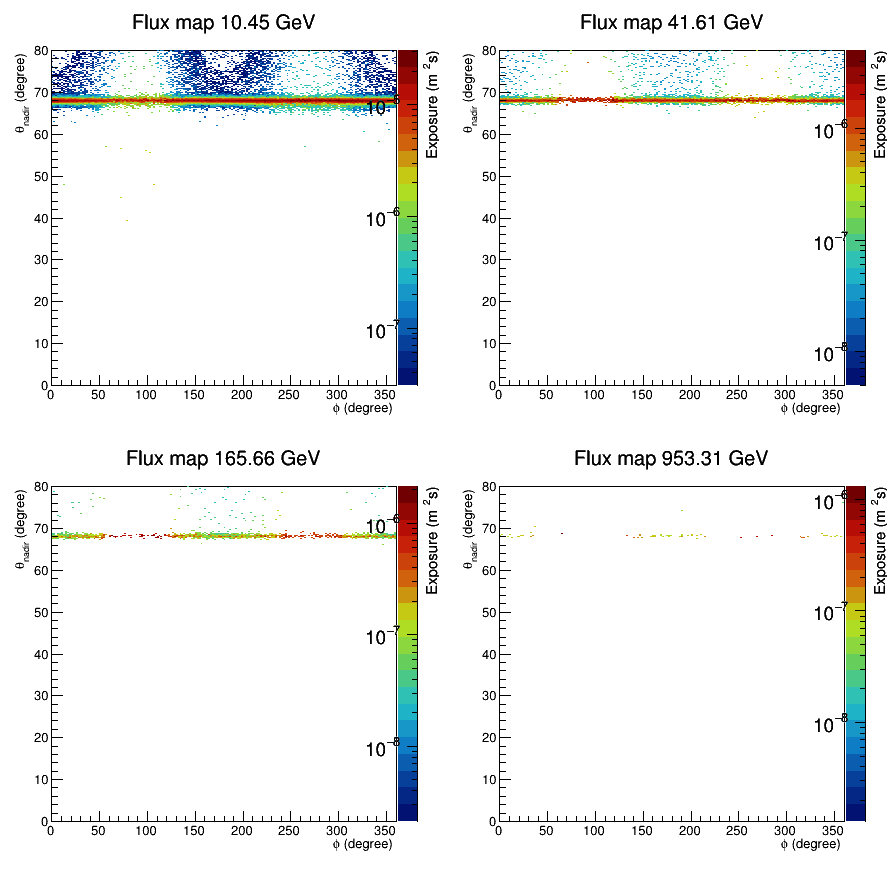
\includegraphics[height=0.9\textheight]{figure/cartesian_flxmaps}};
% \node [opacity=0.2] (0,0) {\rotatebox{45}{\scalebox{3.5}{\textcolor{red}{preliminary}}}};
% \end{tikzpicture}
% \end{figure}
% \end{frame}

% \begin{frame}
% \frametitle{Flux maps}
% \begin{figure}[h!]
% \begin{tikzpicture}
% \node (0,0) {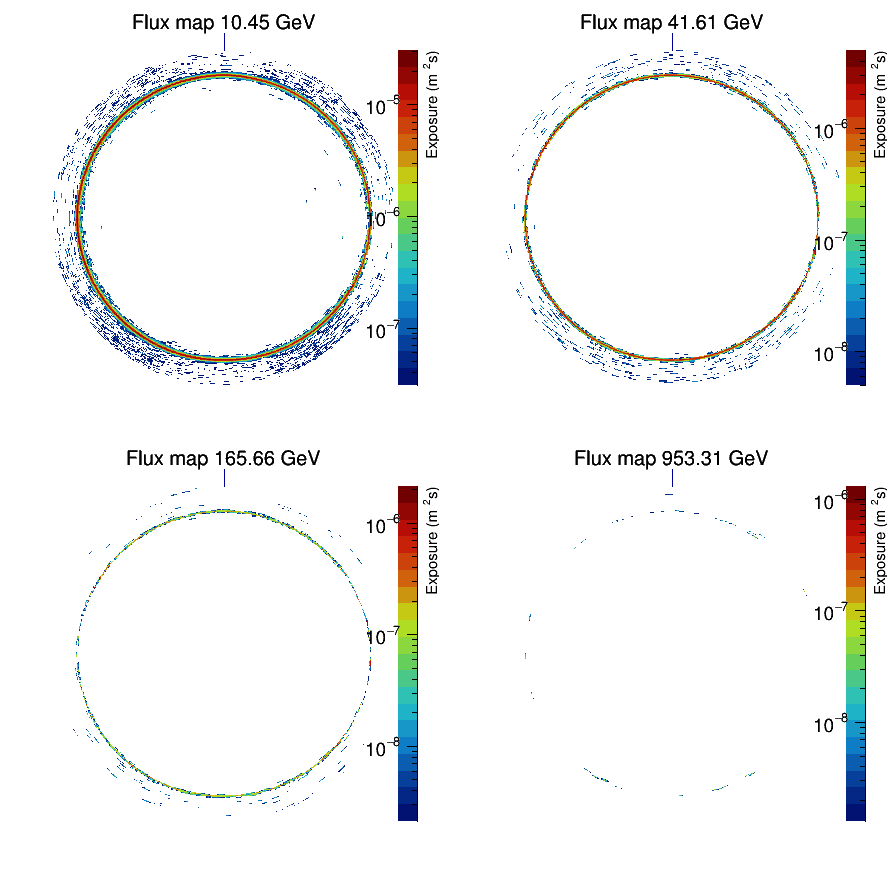
\includegraphics[height=0.9\textheight]{figure/polar_flxmaps}};
% \node [opacity=0.2] (0,0) {\rotatebox{45}{\scalebox{3.5}{\textcolor{red}{preliminary}}}};
% \end{tikzpicture}
% \end{figure}
% \end{frame}


% ------ Monte Carlo Simulation
\begin{frame}
  \frametitle{MC Simulation (Sys. Error): SPL with 200 samplings}
  \begin{figure}[h!]
  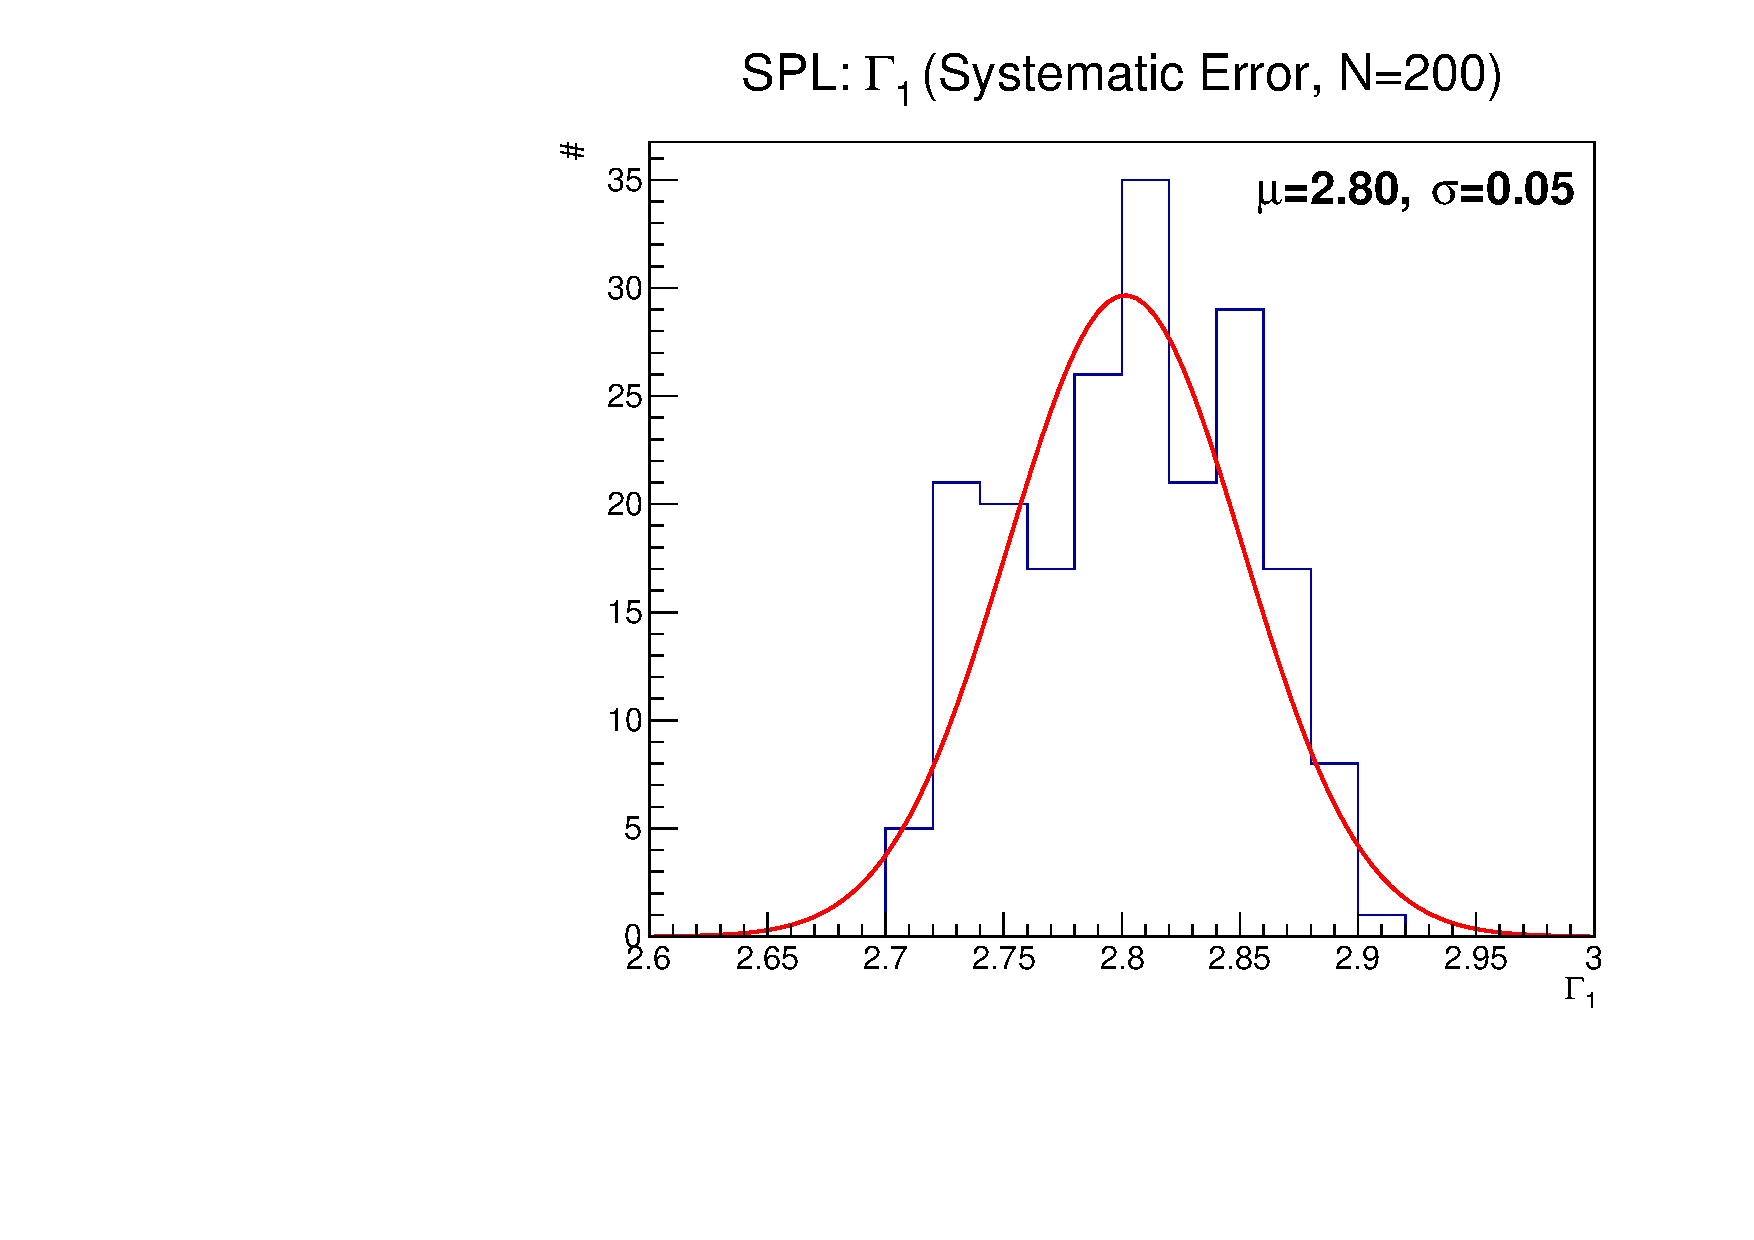
\includegraphics[height=0.8\textheight]{figure/monte_carlo/N200/SPLwHe_gamma1_sys.pdf}
  \end{figure}
\end{frame}

\begin{frame}
  \frametitle{MC Simulation (Tot. Error): SPL with 200 samplings}
  \begin{figure}[h!]
  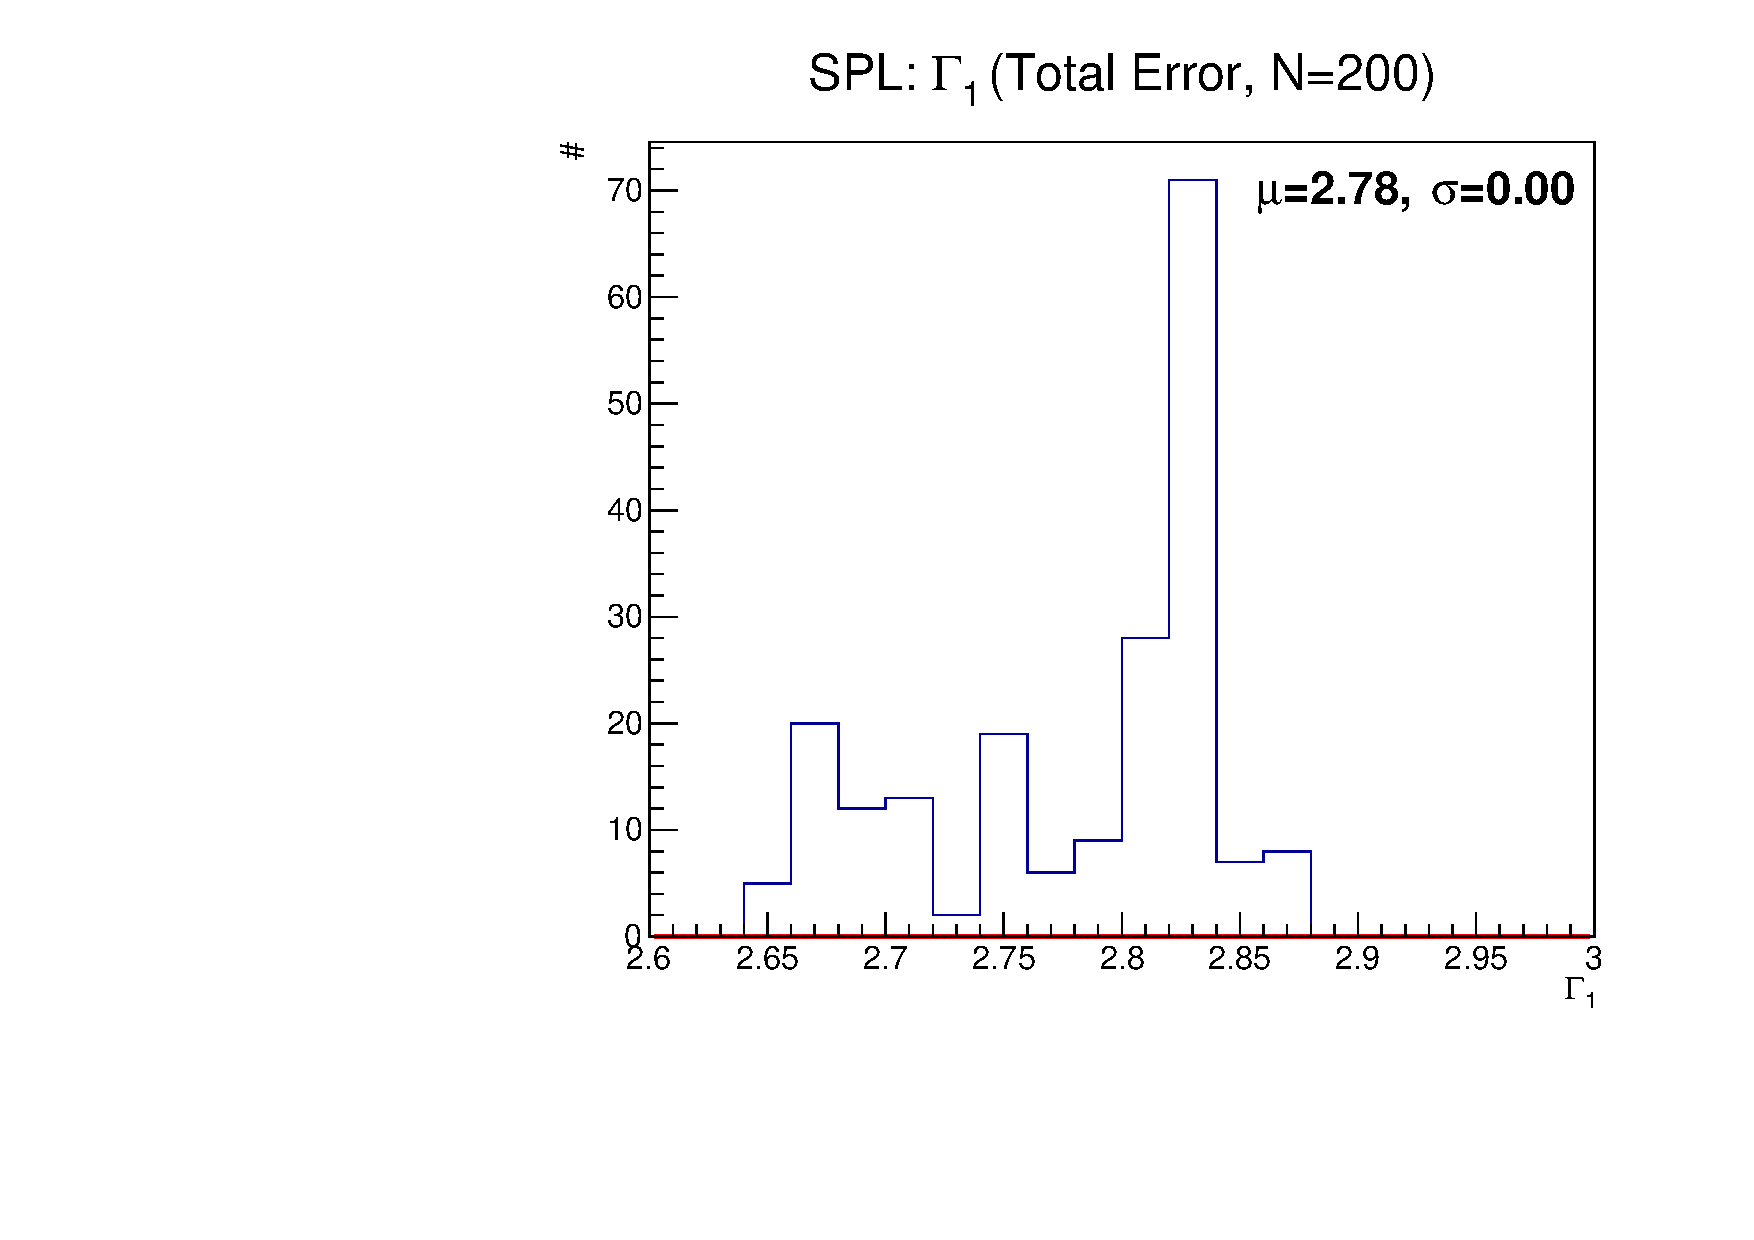
\includegraphics[height=0.8\textheight]{figure/monte_carlo/N200/SPLwHe_gamma1_tot.pdf}
  \end{figure}
\end{frame}


\begin{frame}
  \frametitle{MC Simulation (Sys. Error): BPL with 200 samplings}
  \begin{columns}
    \column{0.33\textwidth}
    \begin{figure}[h!]
      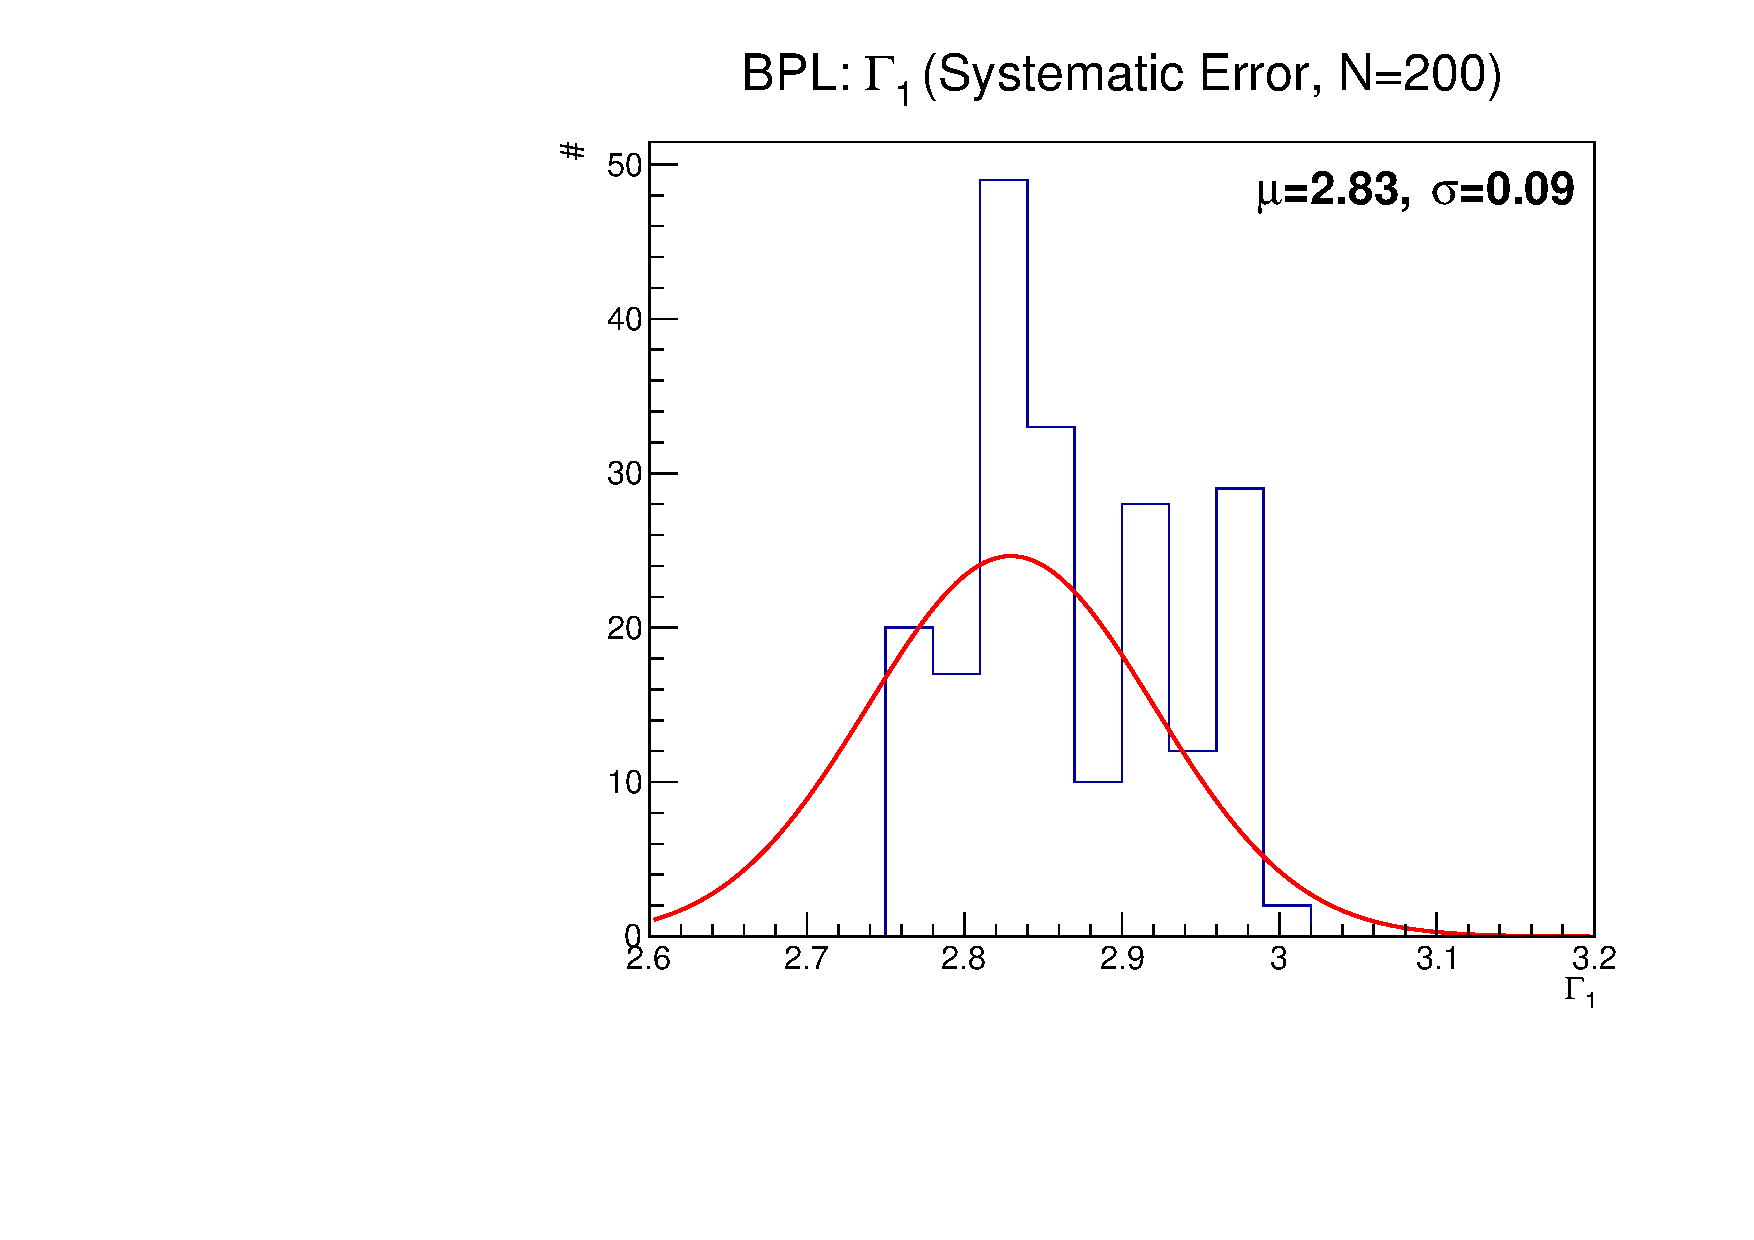
\includegraphics[height=\textwidth]{figure/monte_carlo/N200/BPLwHe_gamma1_sys.pdf}
    \end{figure}
  
    \column{0.33\textwidth}
    \begin{figure}[h!]
      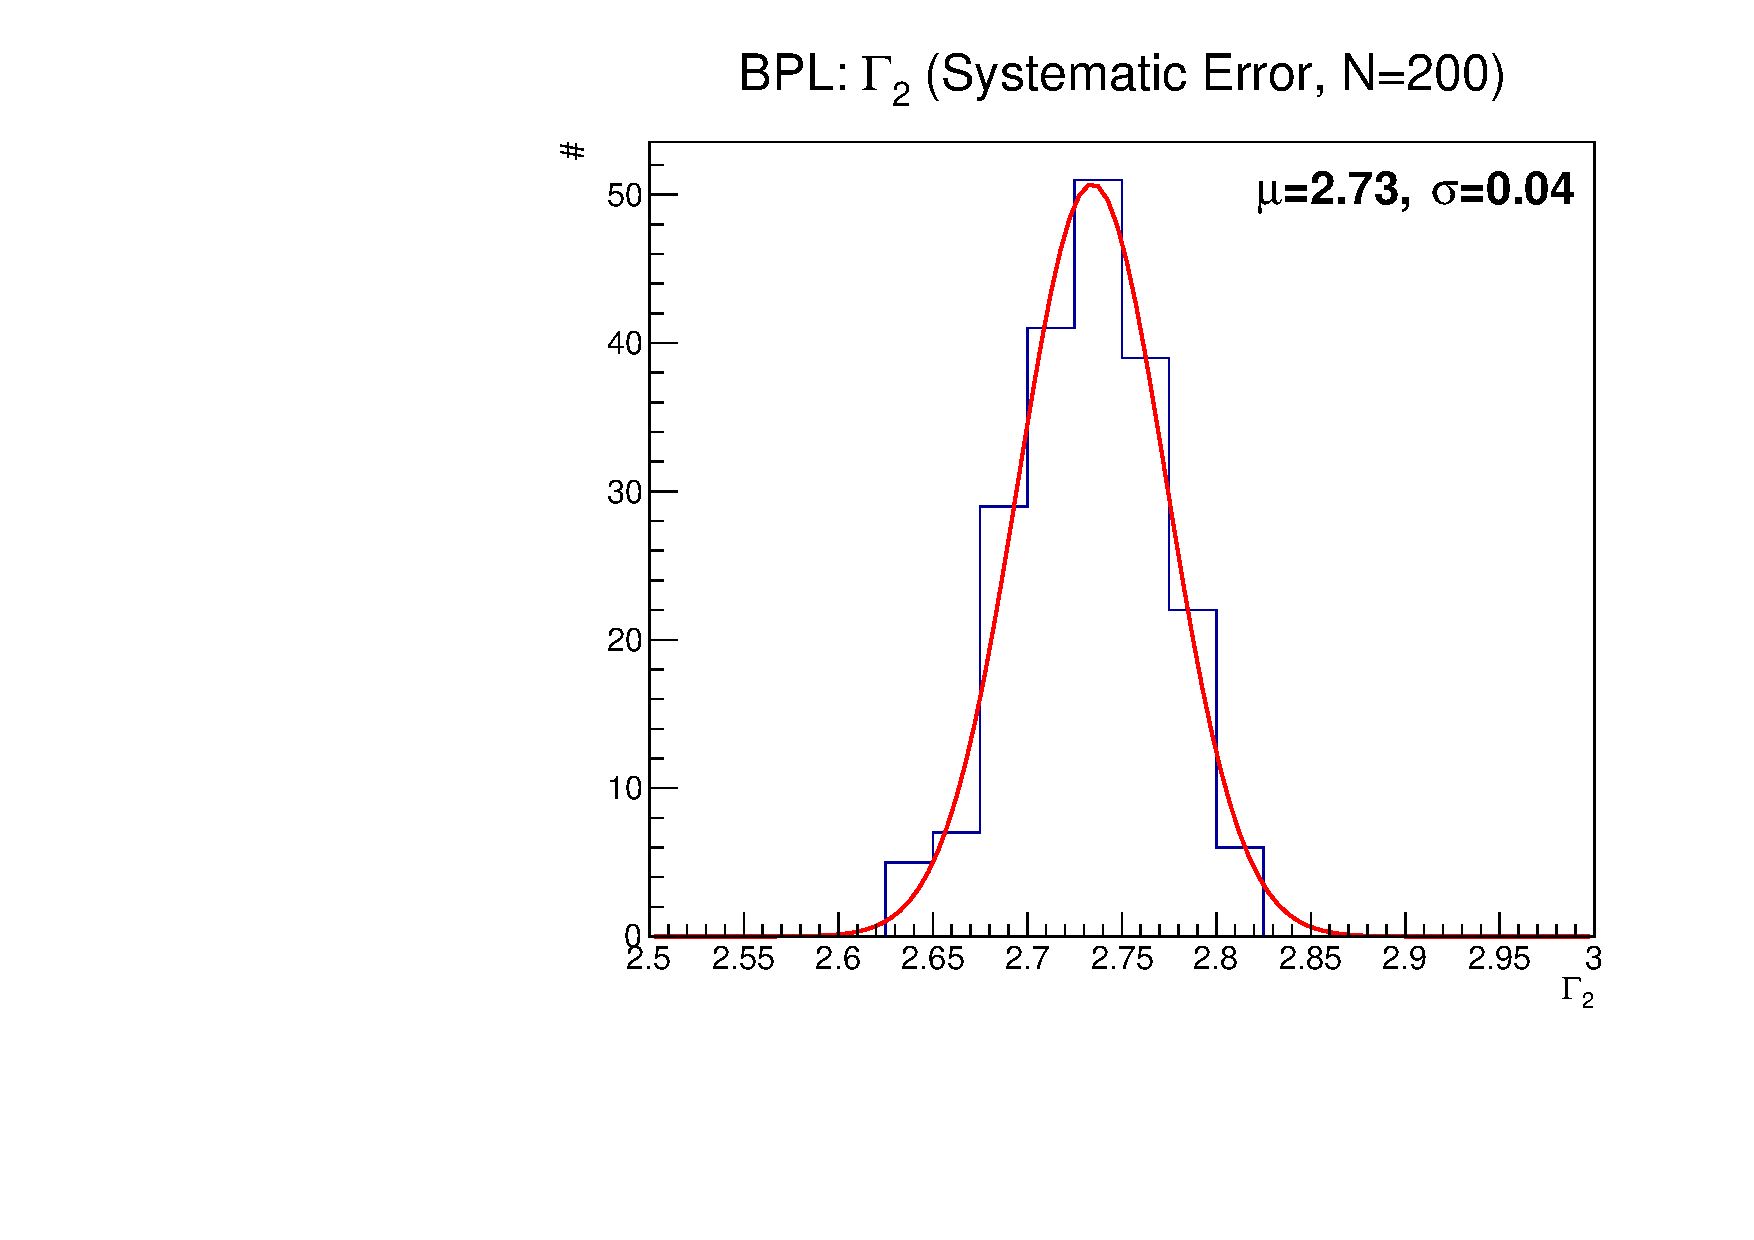
\includegraphics[height=\textwidth]{figure/monte_carlo/N200/BPLwHe_gamma2_sys.pdf}
    \end{figure}

    \column{0.33\textwidth}
    \begin{figure}[h!]
      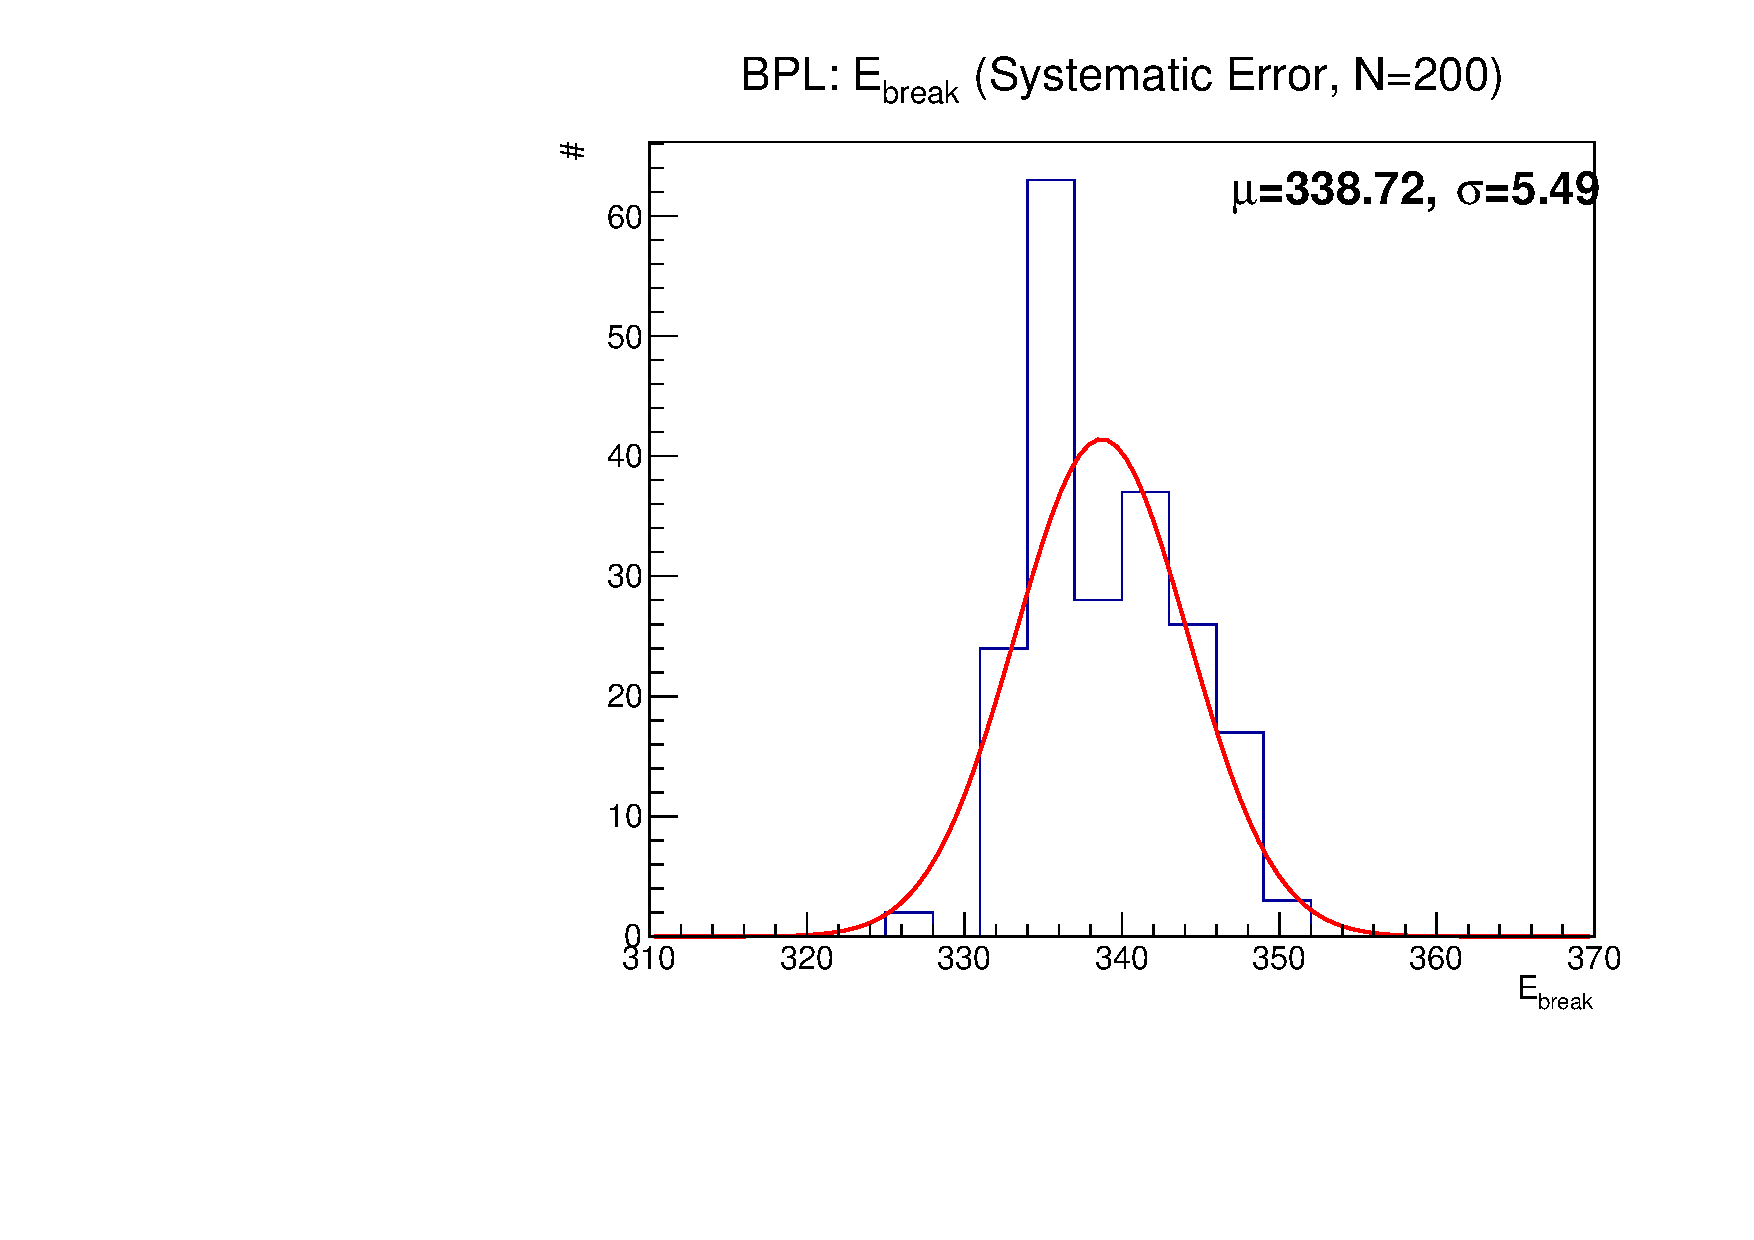
\includegraphics[height=\textwidth]{figure/monte_carlo/N200/BPLwHe_e_break_sys.pdf}
    \end{figure}    
  \end{columns}
\end{frame}


\begin{frame}
  \frametitle{MC Simulation (Tot. Error): BPL with 200 samplings}
  \begin{columns}
    \column{0.33\textwidth}
    \begin{figure}[h!]
      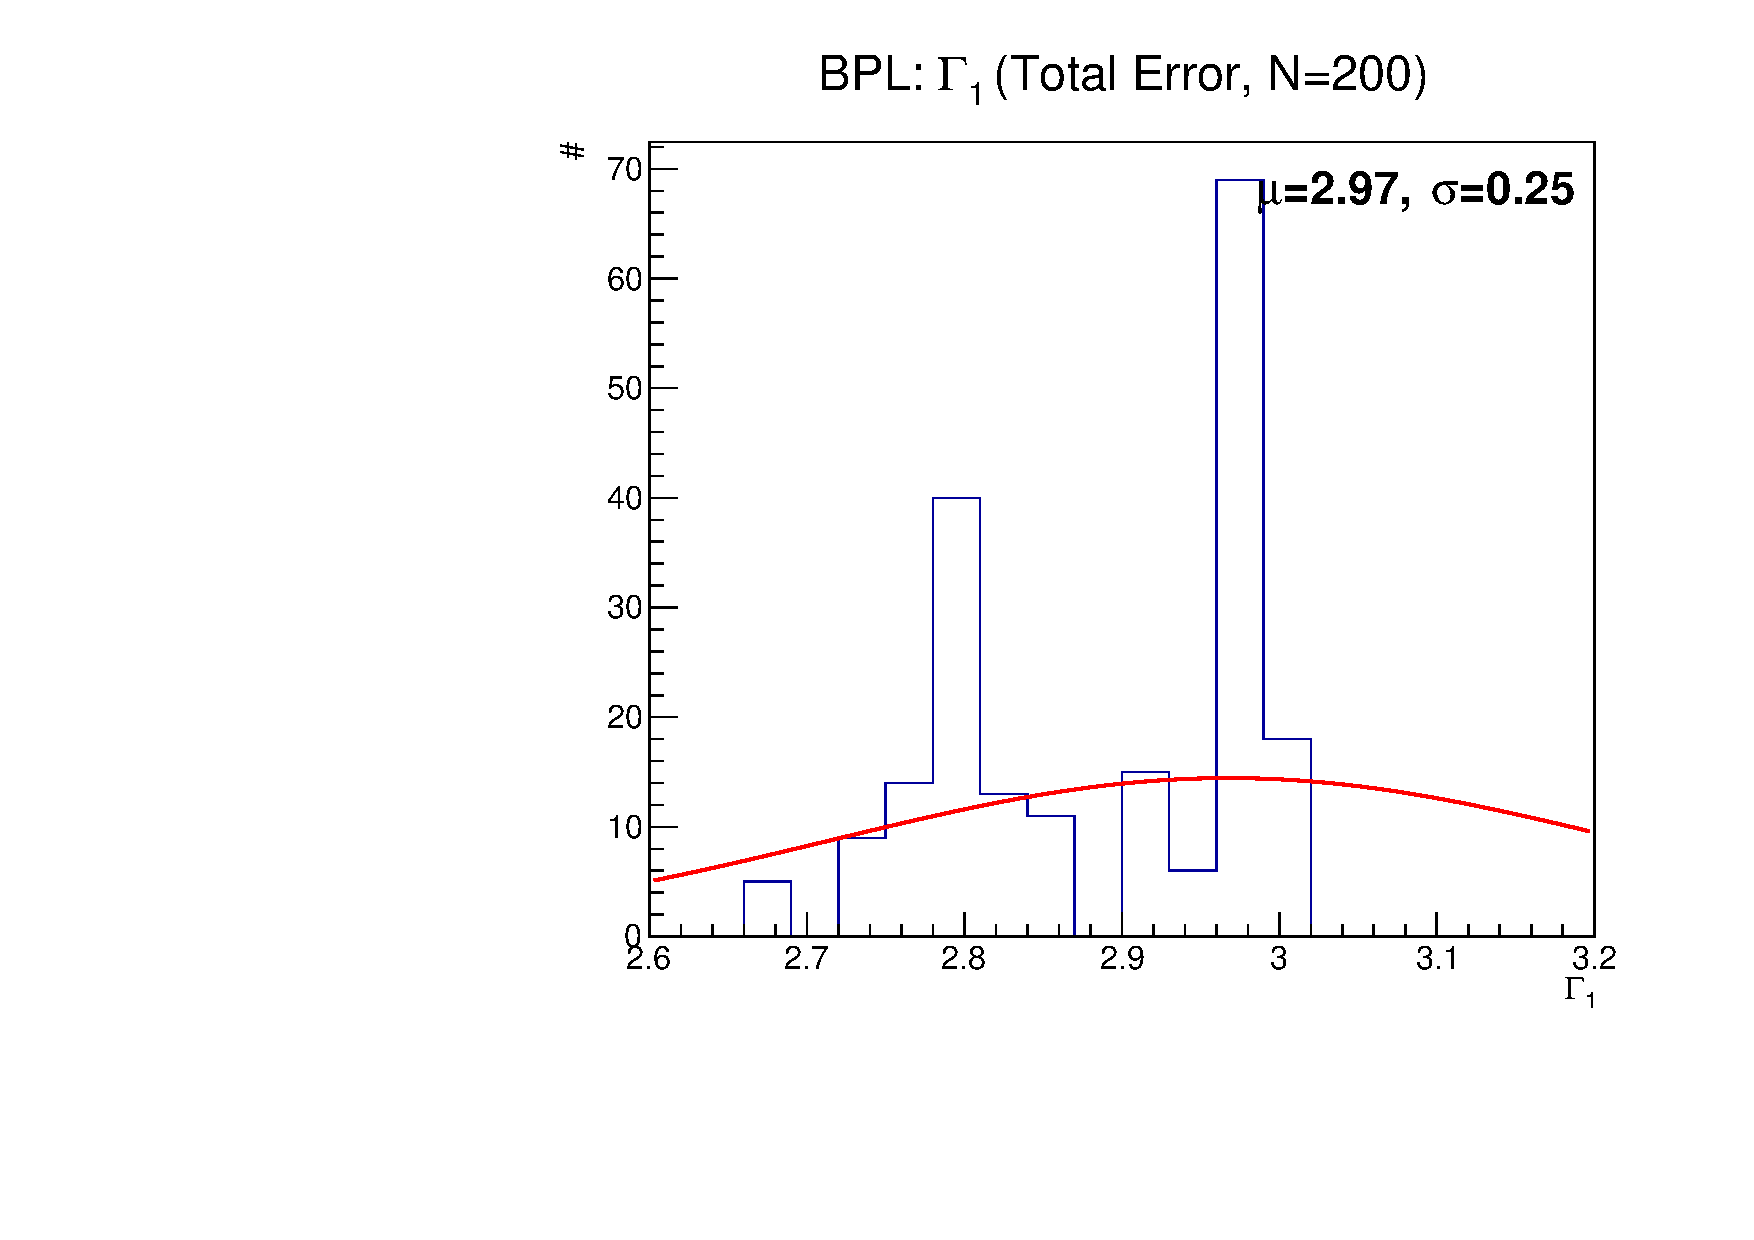
\includegraphics[height=\textwidth]{figure/monte_carlo/N200/BPLwHe_gamma1_tot.pdf}
    \end{figure}
  
    \column{0.33\textwidth}
    \begin{figure}[h!]
      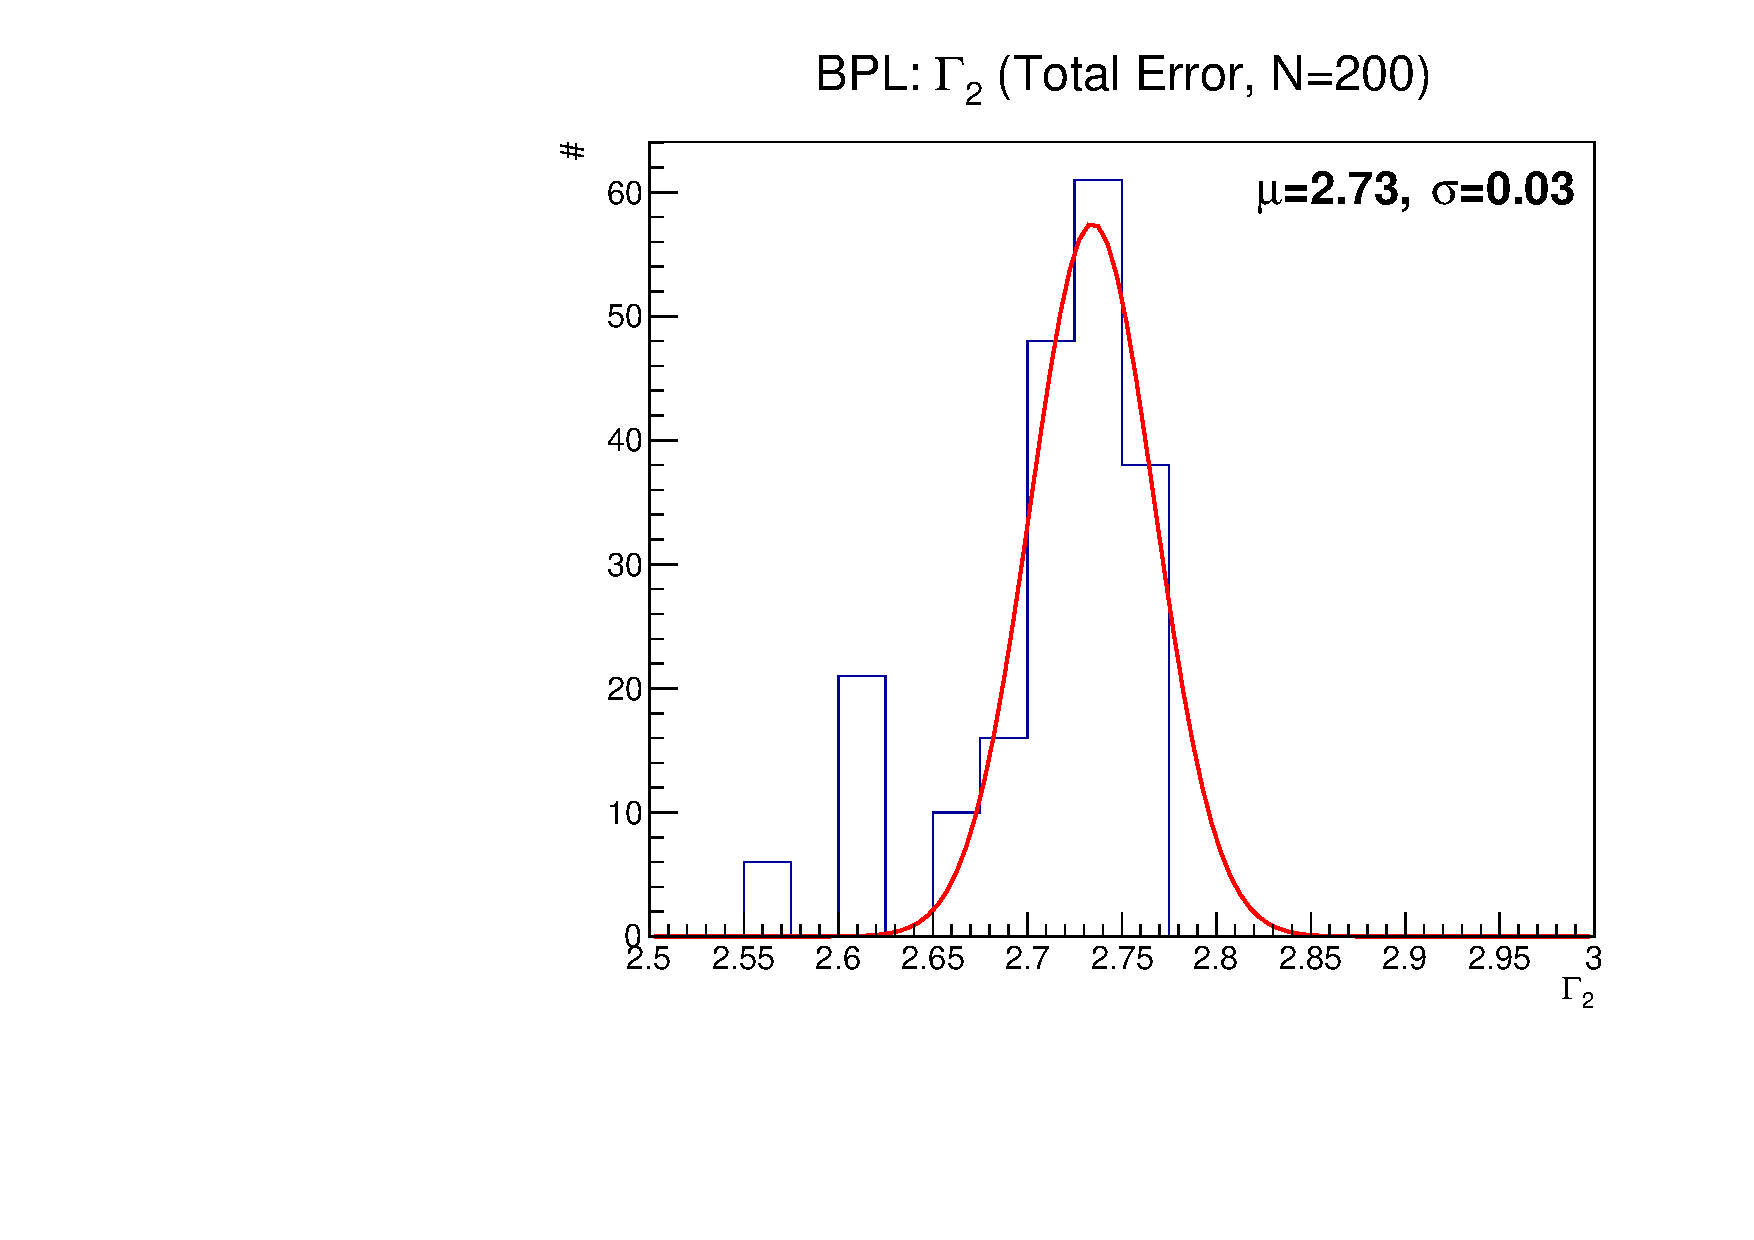
\includegraphics[height=\textwidth]{figure/monte_carlo/N200/BPLwHe_gamma2_tot.pdf}
    \end{figure}

    \column{0.33\textwidth}
    \begin{figure}[h!]
      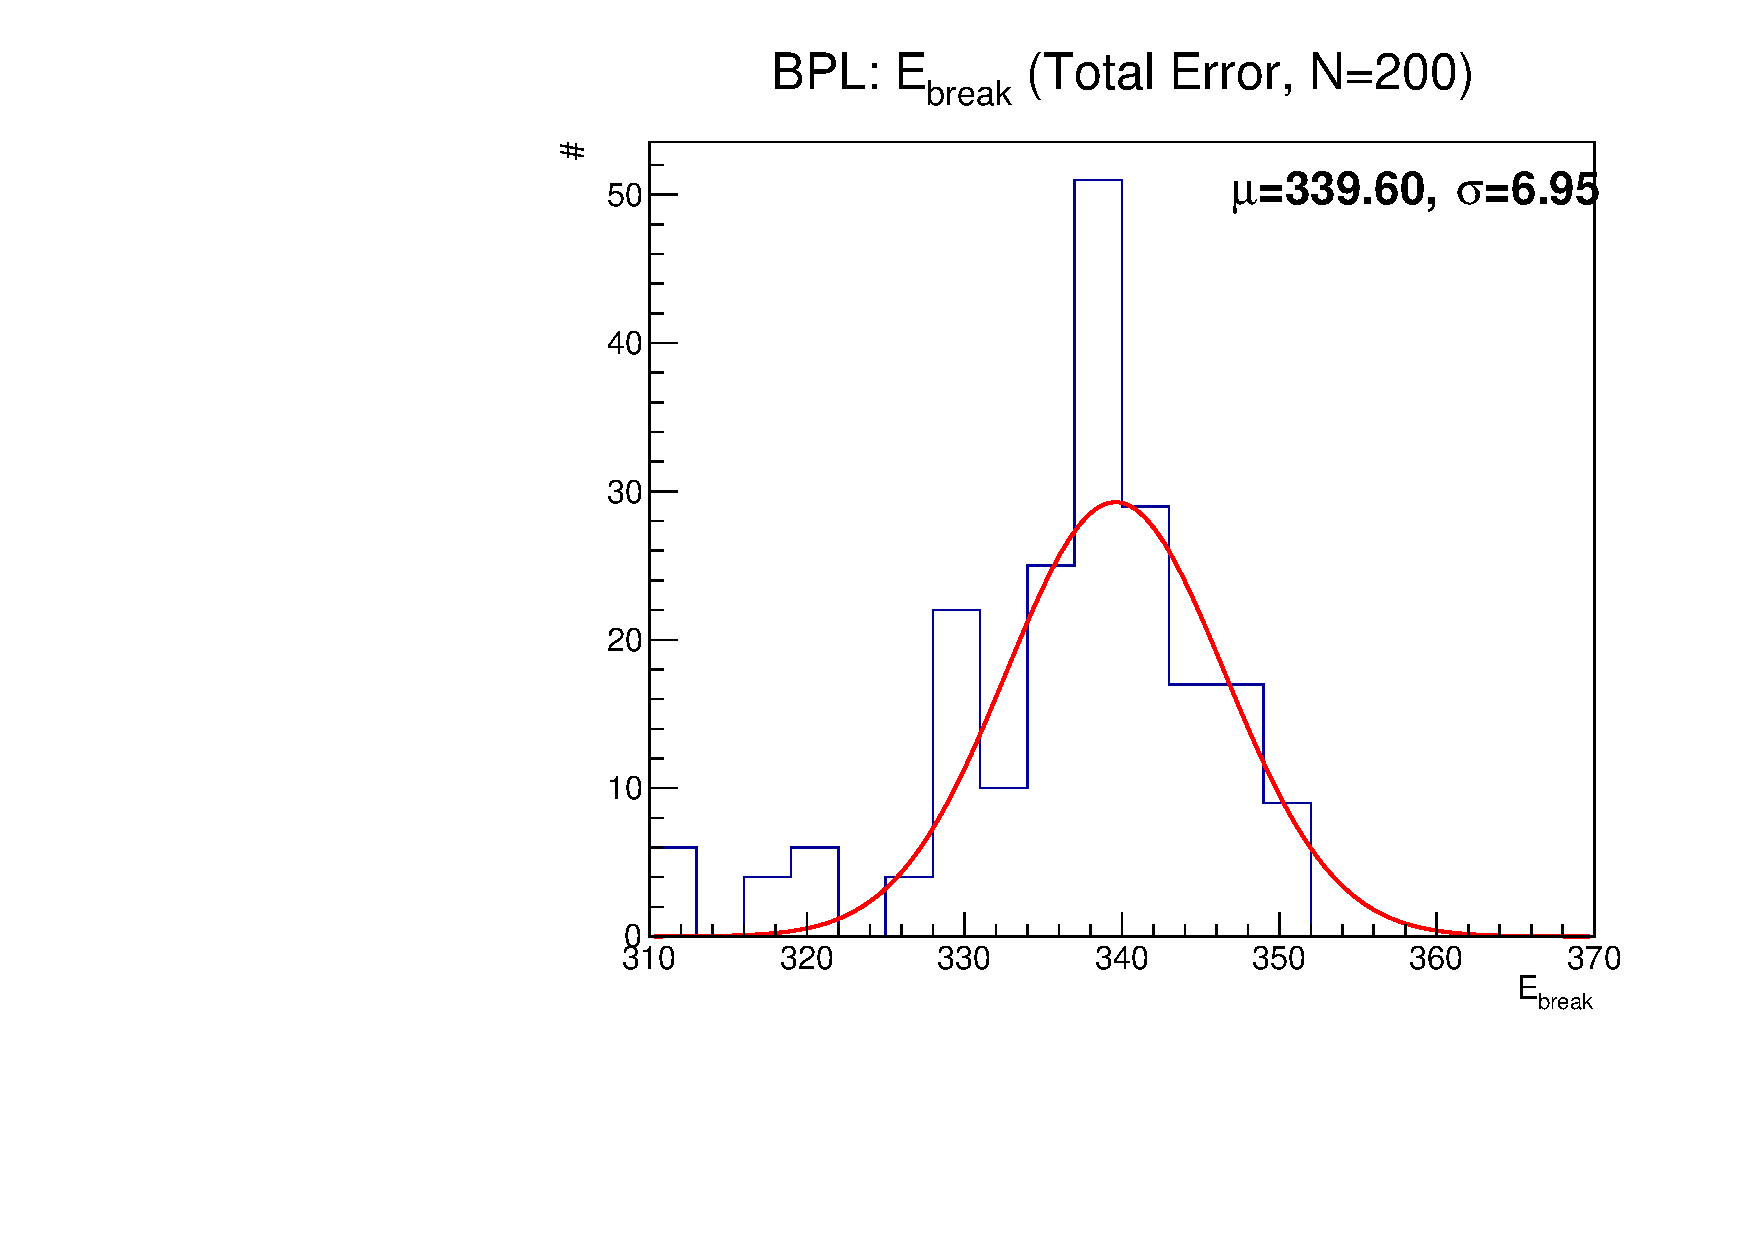
\includegraphics[height=\textwidth]{figure/monte_carlo/N200/BPLwHe_e_break_tot.pdf}
    \end{figure}    
  \end{columns}
\end{frame}

%----------------------------------------------------------------------------------------

\end{document}
